\setchapterpreamble[u]{\margintoc}
\chapter{ModernVBERT: Towards Smaller Visual Document Retrievers}
\label{ch:modernvbert}



\def\flagship{\emph{ModernVBERT}}
\def\flagshipbase{\flagship-base}
\def\flagshipembed{\flagship-embed}
\def\biflagship{\emph{BiModernVBERT}}
\def\colflagship{\emph{ColModernVBERT}}
\def\flagshipparameters{250M}

\newcommand{\cmark}{\ding{51}}% checkmark
\newcommand{\xmark}{\ding{55}}% crossmark

\def\natcap{\textit{NatCap}}
\def\repo{\url{https://huggingface.co/ModernVBERT}}
\def\ghrepo{\url{https://github.com/illuin-tech/modernvbert}}

% Preamble additions:
% \usepackage{booktabs, multirow, makecell, rotating, xcolor, colortbl}
% \usepackage[flushleft]{threeparttable}
\renewcommand\theadfont{\bfseries}
% Define custom colors
\definecolor{grpA}{HTML}{E8F4FF}     % paler blue for group banners
\definecolor{grpB}{HTML}{FFE8EB}     % paler pink for group banners
\definecolor{grpC}{HTML}{E8FFEF}     % paler mint for group banners
\definecolor{grpD}{HTML}{FFF0E0} 
\definecolor{grpE}{HTML}{FFF0F6} 
\definecolor{avgcol}{gray}{0.9}      % avg column grey
\definecolor{dscol}{gray}{0.95}      % dataset name column background
\definecolor{latcol}{RGB}{210,235,255} % light blue for latency column
\definecolor{latcpucol}{RGB}{210,235,255} % light blue (CPU)
\definecolor{latgpucol}{RGB}{170,215,255} % slightly darker blue (GPU)


\begin{sagekaobox}[frametitle=Paper Context]
After the release of ColPali, many Visual Document Retrieval models were trained by various academic and industrial teams around the world, including from our team. Most efforts centered around leveraging stronger VLM backbones which we have shown with the \emph{ColQwen} series to directly improve retrieval performance. 
In this paper released in September 2025 and published at ICML 2026, we instead take another route. With ModernVBERT, we maintain ColPali retrieval performance with a model 10 times smaller. Beyond the ressource release, this paper should be seen as a thorough exploration of the performance factors behind repurposing VLMs for visual embeddings. Our ablations span architecture research, data mixes, cross-modality positive transfers, model souping and more. Importantly, we show strong retrieval performance can be achieved even with little ressources at querying time, enabling cheap deployments and widespread industrial use of the VDR technology.
\end{sagekaobox}


\begin{kaobox}[frametitle=Paper Abstract]
Retrieving specific information from a large corpus of documents is a prevalent industrial use case of modern AI, notably due to the popularity of Retrieval-Augmented Generation (RAG) systems. Although neural document retrieval models have historically operated exclusively in the text space, Visual Document Retrieval (VDR) models - large vision-language decoders repurposed as embedding models which directly work with page screenshots as inputs - are increasingly popular due to the performance and indexing latency gains they offer. In this work, we show that, while cost-efficient, this approach of repurposing generative models bottlenecks retrieval performance. Through controlled experiments, we revisit the entire training pipeline, and establish a principled recipe for improving visual document retrieval models. We notably measure the impact of attention masking, image resolution, modality alignment data regimes, and late interaction centered contrastive objectives which emerge as central performance factors. Building on these insights, we release ModernVBERT, a compact 250M-parameter vision-language encoder that outperforms recent models up to 10 times larger when fine-tuned on document retrieval tasks, enabling efficient inference on cheap CPU hardware and greatly reducing latency and costs while maintaining strong performance. Models, code and data are available at \repo.

\end{kaobox}


\section{Introduction}\label{sec:intro}



\begin{figure}[t]
  \centering
  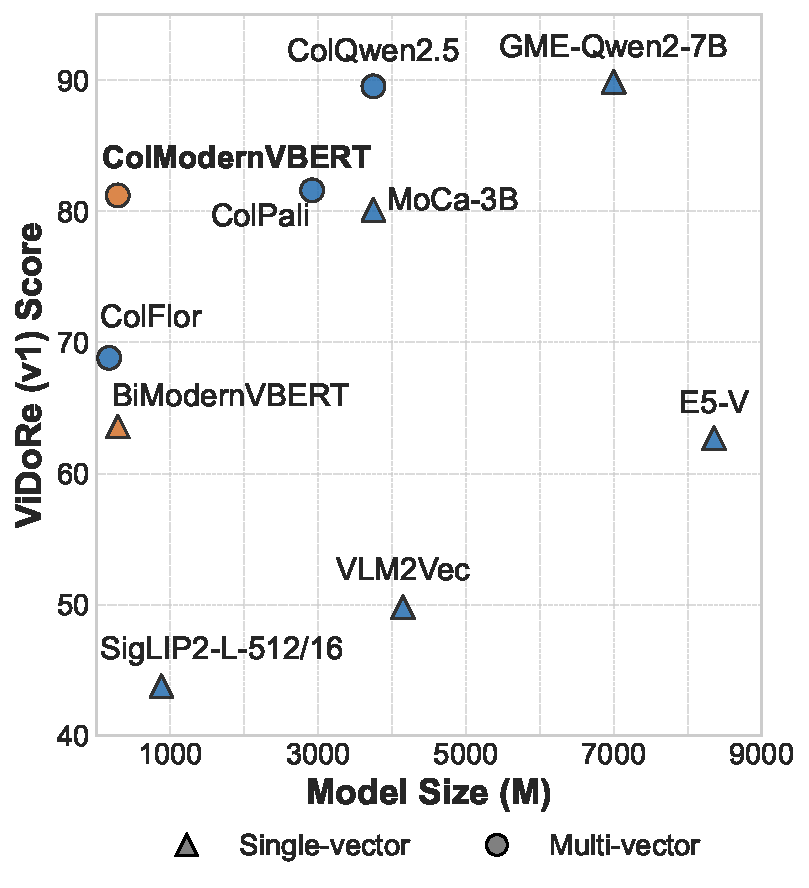
\includegraphics[width=0.88\linewidth]{images/modernvbert_figures/fig_1/pareto_large_models_ColModernVBERT_orange.pdf}
  \caption[Pareto efficiency]{\textbf{Pareto efficiency.} \colflagship{} outperforms models in its category on ViDoRe, achieving a leading performance-size tradeoff.}
  \label{fig:pareto_vidore}
  %\vspace{-10pt}                         % tighten bottom spacing (tweak as needed)
\end{figure}

% Context paragraph
% this is colpali's first paragraph, nice start point but to be modified. I think the reviewer is right in the sense that let's not overcomplicate the first paragraph. in the end its VDR so let's simply motivate it. @manu, c'est un draft fais toi plaisir, jen suis pas 100% convaincu de la forme mais j'aime le fond
% \textcolor{red}{Visual Document Retrieval (VDR) is a recently introduced alternative to text-based search systems, which, given a user query, consists in identifying relevant document pages within a large corpus by relying on their image screenshots rather than their pre-extracted textual content \sidecite{faysse2025colpaliefficientdocumentretrieval}. 
%Applications of Retrieval Augmented Generation (RAG) \sidecite{lewis_retrieval-augmented_2020} are ubiquitous in the industry, but remain bottlenecked by the quality of the first-stage retrieval system. To process documents such as PDFs, for many years, the standard approach was to extract the textual information of the documents--relying on OCR modules--and perform retrieval in the text space \sidecite{lin-byrne-2022-retrieval}.} Owing to the performance improvements enabled by generative vision–language models (VLMs), recent work has increasingly explored \textcolor{red}{operating in the vision space instead}, repurposing these models as multimodal encoders through extended contrastive post-training~\sidecite{ma2024unifyingmultimodalretrievaldocument, faysse2025colpaliefficientdocumentretrieval, jiang2024vlm2vectrainingvisionlanguagemodels}.

The ability to quickly locate specific information in vast document collections is a core building block of digital systems today, supporting use cases that range from web search and virtual assistants to enterprise knowledge management. Neural information retrieval (IR) models, and in particular dense retrievers, have become the de facto backbone of modern search systems thanks to their strong semantic matching capabilities and good scalability properties \sidecite{reimers2019sbert, karpukhin2020dpr, wang_text_2022}.  

This trend is amplified by the widespread adoption of Retrieval-Augmented Generation (RAG) \sidecite{lewis_retrieval-augmented_2020}, where a retriever is used to select a small set of relevant documents that condition a downstream generator. In such systems, the first-stage retrieval module is a well-known bottleneck: its recall directly upper-bounds the quality of the generated answers, while its latency and indexing costs partially drive the overall system efficiency \sidecite{lin-byrne-2022-retrieval}. As a result, improving document retrieval, especially for long, complex files such as PDFs, scientific articles, and reports, is a key lever for making industrial RAG deployments more accurate and cost-effective.
% \begin{wrapfigure}[24]{tr}{0.52\textwidth} % <- 12 = approx. number of text lines to wrap
%   \vspace{-5pt}                          % tighten top spacing (tweak as needed)
%   \centering
%   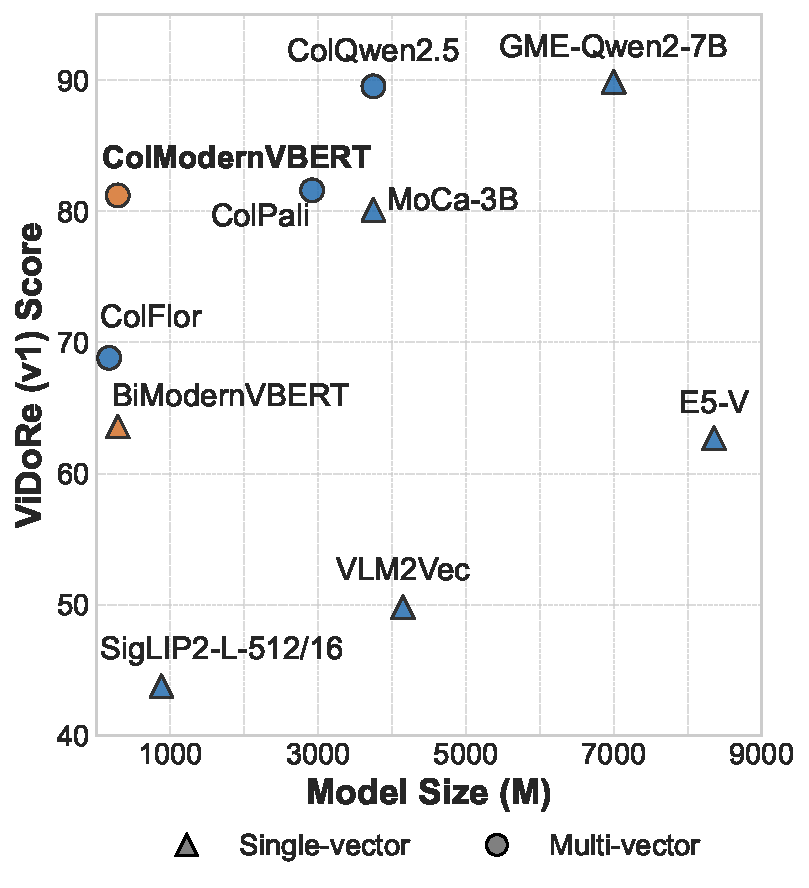
\includegraphics[width=\linewidth]{images/modernvbert_figures/fig_1/pareto_large_models_ColModernVBERT_orange.pdf}
%   \caption{\textbf{Pareto efficiency.} \colflagship{} outperforms models in its category on ViDoRe, achieving a leading performance-size tradeoff.
%   }
%   \label{fig:pareto_vidore}
%   %\vspace{-10pt}                         % tighten bottom spacing (tweak as needed)
% \end{wrapfigure}

\textbf{Visual Document Retrieval.} Historically, document retrieval in these settings has operated purely in the text space. To index PDFs or scans, practitioners first run heavy preprocessing pipelines that include Optical Character Recognition (OCR), layout analysis, and heuristic passage segmentation, before embedding the resulting text spans with a neural encoder. 
% \begin{wrapfigure}[23]{tr}{0.5\textwidth} % <- 12 = approx. number of text lines to wrap
%   \vspace{-5pt}                          % tighten top spacing (tweak as needed)
%   \centering
%   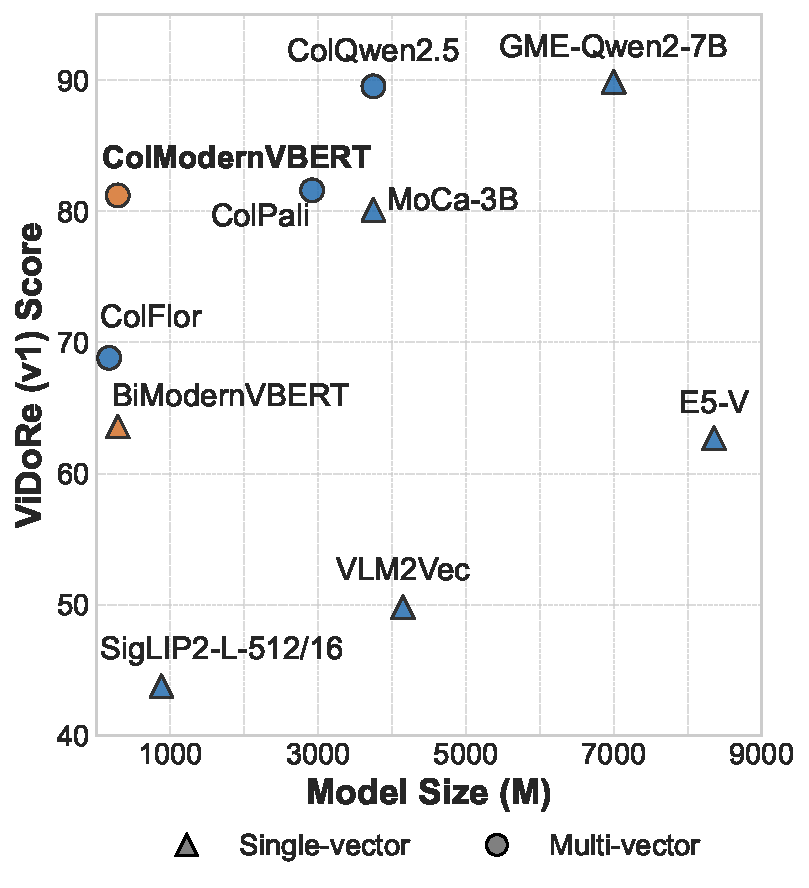
\includegraphics[width=\linewidth]{images/modernvbert_figures/fig_1/pareto_large_models_ColModernVBERT_orange.pdf}
%   \caption{\textbf{Pareto efficiency.} \colflagship{} outperforms models in its category on ViDoRe, achieving a leading performance-size tradeoff.
%   }
%   \label{fig:pareto_vidore}
%   %\vspace{-10pt}                         % tighten bottom spacing (tweak as needed)
% \end{wrapfigure}
This approach suffers from several limitations: OCR and layout parsing can be brittle and slow, complex visual elements such as tables, figures, and typography are often poorly captured, and any error or bias introduced during preprocessing is propagated to the retriever. % Recent work has shown that these multi-stage text pipelines can underutilize the rich visual structure of documents and leave significant performance on the table, especially in visually intensive domains \sidecite{faysse2025colpaliefficientdocumentretrieval}. 

\textit{Visual Document Retrieval} (VDR) has emerged as a compelling alternative to such text-based systems. Rather than indexing pre-extracted textual content, VDR models directly operate on page screenshots: given a user query, they retrieve relevant document pages by matching the query against image-based representations of the pages \sidecite{faysse2025colpaliefficientdocumentretrieval}. By bypassing OCR and layout parsing, VDR yields simpler end-to-end pipelines, significantly reduces indexing latency, and better exploits visual cues such as layout, figures, and fonts, while achieving strong performance on visually rich benchmarks like ViDoRe. 

\textbf{Limits of Generative VLM Repurposing.} Most current VDR systems are obtained by repurposing large generative vision–language decoders ~\sidecite{alayrac_flamingo_2022} as retrieval encoders via post-hoc contrastive fine-tuning \sidecite{ma2024unifyingmultimodalretrievaldocument, faysse2025colpaliefficientdocumentretrieval, jiang2024vlm2vectrainingvisionlanguagemodels}. While cost-efficient, this design choice bottlenecks retrieval performance and efficiency: model sizes, attention patterns, image resolutions, and training objectives are designed for generative use cases rather than optimized for retrieval which has been shown in text models to be suboptimal \sidecite{lee2024nvembedimprovedtechniquestraining, gisserotboukhlef2025pretrainencodersmaskedlanguage}. Furthermore, scaling trends \sidecite{wei2022emergentabilitieslargelanguage} are less pronounced for embedding models; while correlated with model size, strong retrieval performance remains attainable with small models \sidecite{clavié2024bettermonolingualjapaneseretrievers}.

% Learning rich embeddings aligned between text and image modalities remains a central challenge in visual retrieval.
% A core challenge in visual retrieval is learning text–image embeddings that faithfully encode complex, multi-level semantics—from fine-grained details to high-level concepts.
% For many years, \emph{contrastive pre-training} of dual encoders, typically pairing a vision transformer (ViT)~\sidecite{dosovitskiy_image_2020} with a text encoder, was the standard approach for generating cross-modal embeddings~\sidecite{radford_learning_2021, zhai_sigmoid_2023}. Owing to the performance improvements enabled by generative vision–language models (VLMs), recent work has increasingly explored repurposing these models as multimodal encoders through extended contrastive post-training~\sidecite{ma2024unifyingmultimodalretrievaldocument, faysse2025colpaliefficientdocumentretrieval, jiang2024vlm2vectrainingvisionlanguagemodels}. 






% While this approach capitalizes on the inherent capabilities of the backbone generative model to address complex visual tasks~\sidecite{alayrac_flamingo_2022}, it is unclear whether the design decisions made for generative purposes hinder the models when repurposed for representation learning. 
% Typically, generative VLMs are built as vision extensions to Large Language Models designed for autoregressive generation, often with a focus on strong knowledge and reasoning skills.

% Typically, VLM-based encoders inherit the causal attention masks VLMs are trained with, which has been repeatedly shown to be suboptimal for embedding tasks~\sidecite{li2023generaltextembeddingsmultistage, behnamghader_llm2vec_2024, lee2024nvembedimprovedtechniquestraining, springer2025repetitionimproveslanguagemodel, gisserotboukhlef2025pretrainencodersmaskedlanguage}. 



% Another notable architectural property of contemporary VLMs is their high parameter counts. LLMs exhibit emergent abilities in reasoning and knowledge use as they grow in size \sidecite{wei2022emergentabilitieslargelanguage}, and most openly released decoders and their vision-augmented variants are at least several billion parameters. Interestingly, scaling trends are less pronounced for embedding models: while size remains a performance factor, compact encoders often almost rival the performance of much larger ones, indicating diminishing returns with additional parameters \sidecite{muennighoff_mteb_2022}. 
% Visual retrieval benchmarks such as ViDoRe and MIEB ~\sidecite{xiao2025miebmassiveimageembedding} are no exception, and model sizes within a same model family has been shown to deliver clear, but limited gains. Taken together, this 

% This suggests it is likely possible to achieve strong visual representation quality with relatively small, well-trained models, especially leveraging late interaction methods \sidecite{clavié2024bettermonolingualjapaneseretrievers}.



% What are we doing?
% \manu{Important not to be redundant with contributions detailed later on. --> In this paper, we opt to build document retriever models from the ground up, freeing ourselves from the constraints of strating from repurposed VLMs. Our contributions are the following:}
% \noindent\textbf{Revisiting Design Decisions in VLM Decoder Embedder Models.} 
% \manu{would be nice to introduce a bit more about the fact we are conducting controlled ablations. somethikgn along the line of - principled ablatioons have been done for vision models, for text models but not for vlms which are recent. this paper fills the gap. One thing we could put some emphasis on is how we "selected" the modality alignement mix to particularly be interesting for document retrieval (whether this is true or false, we make it sound like that. another key point is modality transfer for contratsive which is a cool "princiupled"result }
Recent papers and model releases in the visual retrieval space have claimed performance improvements by scaling the amount of contrastive data and the compute budget \sidecite{zhang2025gmeimprovinguniversalmultimodal, xu2025llamanemoretrievercolembedtopperforming}, modifying the attention mask \sidecite{chen2025mocamodalityawarecontinualpretraining}, increasing image resolutions \sidecite{cohere_introducing_2024} or by introducing more diverse tasks and data sources \sidecite{jiang2024vlm2vectrainingvisionlanguagemodels}. %Furthermore, it remains unclear whether the performance gains offered by these models are due to improved image representation capabilies or rather are enabled by aligned text and visual latent spaces.

% In this work, we revisit the entire training pipeline for visual document retrieval through controlled experiments, identify key design factors for effective VDR (including attention masking, image resolution, modality alignment data regimes, and late-interaction–centric contrastive objectives), and introduce ModernVBERT, a compact 250M-parameter vision–language encoder that outperforms recent VDR models up to ten times larger on document retrieval tasks, while enabling efficient inference on cheap CPU hardware.


In this work, we attempt to centralize these efforts and systematically disentangle the impact of core design decisions in visual retriever training. 
% Through rigorous experimentation in controlled setups, starting from language model pretraining to multi-stage domain specific finetuning, we attempt to identify: \textit{What makes a visual retriever great?} 
% By systematically disentangle the impact of core design choices in visual retriever training. 
Through controlled experiments—ranging from language model pretraining to multi-stage, domain-specific fine-tuning, we aim to answer a central question:
% \anto{On ne fait pas vraiment de language model pretraining - non mais on conbtrole pour ca}

\begin{center}
\textit{Which design choices best boost performance in modern visual document retrievers?}
\end{center}

% In this work, we take a principled approach ourselves how to best train a visual encoder from the ground up - freeing ourselves from the constraints of starting from pretrained VLMs. Our contributions are the following:

% \noindent\textbf{Contribution 1.}\; We critically reassess the core assumptions in multimodal encoder design. Contrary to the prevailing view, \textit{our analyses show the main strength of VLM-based encoders is not better image embeddings, but stronger alignment between image and text token embeddings}. Through controlled experiments, we measure the role of alignment length, training duration, and cross-modality interactions. We show alignment effectiveness is task-dependent, and provide evidence that causal attention is suboptimal in visual document retrieval, especially with late interaction~\sidecite{khattab2020colbert, faysse2025colpaliefficientdocumentretrieval}. \manu{something about causal attention here would make sense maybe ?}

% \manu{Is this still a contribution ? do we want to back up these claims ? esp. if the claims are document leaning ?}
% \noindent\textbf{Contribution 2: \natcap{}.}\; Existing contrastive datasets consist mainly of web-collected image–caption pairs or image–label pairs. Yet these pairs are often either too general (generic captions) or too narrow (single labels), lacking the contextual richness available in backbone LMs. To address this, we introduce \natcap{}, a contextualized image–caption dataset. We synthetically generate captions from classification training sets by providing the model with the image, its label, and task metadata as context. Through dataset ablations, we show that \natcap{} can be particularly beneficial for zero-shot classification tasks.

% \noindent\textbf{Contribution 3: \flagship{}.}\; Building on these insights, we design and release \flagship{}, \paul{double check this} the first multimodal encoder that aligns a pretrained language model encoder with a CLIP vision tower through Masked Language Modeling (MLM) objective. \paul{check ce qui suit avec les resultats} Despite its modest size and low data regime \manu{why low data regime ? prefer something like modest training budget}, this encoder outperforms \manu{give scale} larger VLM-based models on document retrieval while remaining competitive on natural image benchmarks \manu{the competitive natiure of ilages is something we want to claim ?}. Our results demonstrate that strong, efficient vision encoders can be obtained without the excessive parameter counts and architectural limitations of repurposed generative VLMs.

%\noindent\textbf{Contribution 1.}\; We revisit core assumptions in visual retriever design, showing that token-level objectives—beyond coarse contrastive alignment—are main drivers of retrieval performance, and that beyond strong image features, overlooked gains lie in improved fine-grained image–text alignment. We further show that causal attention is suboptimal in document retrieval, with bidirectional masking offering clear improvements in multi-vector settings, and that other parameters such as image resolution data mixes should not be overlooked in the training pipeline.

\noindent\textbf{Contribution 1.}\; We revisit core assumptions in visual retriever design, showing that token-level training objectives benefit retrievers by strengthening image–text token alignment—rather than merely producing stronger image embeddings.
Our results indicate that causal attention is suboptimal in document retrieval, with bidirectional masking offering clear improvements in multi-vector settings, and that other parameters such as image resolution data mixes should not be overlooked in the training pipeline.

% \noindent\textbf{Contribution 1.}\; We revisit core assumptions in visual retriever design. 
% % Token-level objective improves visual document retrieval performance
% We observe that token-level objectives consistently enhance document retrieval performance, and that beyond the use of strong image features, early fusion models yield overlooked benefits through improved fine-grained image–text alignment.
% % Causal attention is suboptimal in visual document retrieval, bidirectional attention unlock full potential of late inetraction, and other parameters such as image resolution and data mixes should not be overlooked.
% We further show that causal attention is suboptimal in visual document retrieval, with bidirectional masking offering clear improvements, and that other parameters such as image resolution data mixes should not be overlooked in the training pipeline.

% \noindent\textbf{Contribution 1.}\; We revisit core assumptions in visual retriever design. Notably, we show that causal attention is suboptimal in multi-vector document retrieval, with bidirectional masking offering clear improvements as a counterpart. We further show that token-level objectives—beyond coarse contrastive alignment—are important drivers of retrieval performance, and that beyond strong image features, overlooked gains lie in improved fine-grained image–text alignment.

%We critically reassess the core assumptions in visual retriever design. 

%We show that token-level objectives are beneficial in document retrievers training, and that contrary to the prevailing view, the main strength of VLM-based encoders is not better image embeddings, but stronger alignment between image and text token embeddings due to this token-level training objective. 

%We provide evidence that \textit{causal attention is suboptimal for visual retrieval tasks, especially in multi-vector settings}. Like in generative tasks, we observe that visual document retrieval is resolution-sensitive, 

%and that a cooldown on high-resolution images during modality alignment can improve model performances in such tasks.

\noindent\textbf{Contribution 2: \flagship{}.}\; Building on these insights, we release \flagship{}, a small \flagshipparameters{} multimodal encoder that aligns a pretrained language encoder with a vision encoder through Masked Language Modeling (MLM) objective, and \colflagship{} a variant fine-tuned for document retrieval. Despite its modest size and limited training budget, \colflagship{} matches models 10x larger on standard visual document retrieval benchmarks, demonstrating the interest of designing a retrieval focused model from the ground up. 
% We publicly release the model, intermediate checkpoints, and the training code at \repo{}.
We release the model, intermediate checkpoints, and the training code at \repo.

% Our results demonstrate that performant vision retrievers can be obtained without the excessive parameter counts and architectural limitations of repurposed generative VLMs.

% \begin{figure}[ht]
%     \centering
%     \includegraphics[width=0.6\textwidth]{example-image.png}
%     \caption{\paul{TODO} \manu{This could also be a table about what the different ablations taught us (green checkmarks, red crosses. Pareto might be too childish}}
%     \label{fig:pareto_frontier}
% \end{figure}

% \begin{figure}[t]
%     \centering
%     \includegraphics[width=\linewidth]{images/modernvbert_figures/fig 1/vbert_visu_fig1.pdf}
%     \label{fig:schema_causal_bidir}
%     \caption{\paul{TODO}}
% \end{figure}

% \begin{figure}[t]
%     \centering
%     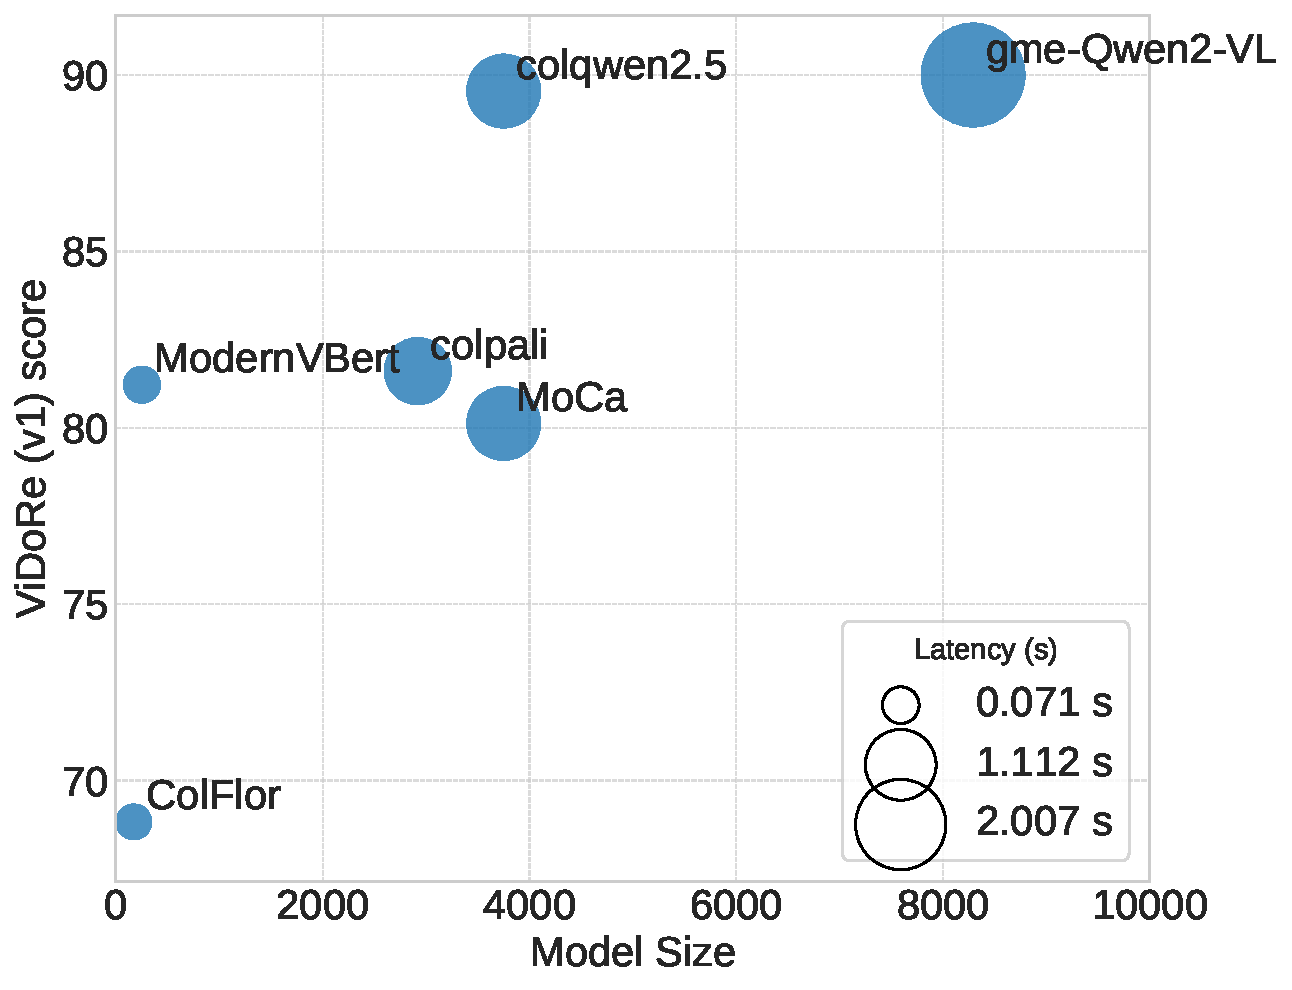
\includegraphics[width=0.5\linewidth]{images/modernvbert_figures/pareto_plot.pdf}
%     \label{fig:pareto}
%     \caption{\paul{TODO}}
% \end{figure}


% We show The primary advantage of modality alignment methods (MLM/CLM objectives) lies not in improved intrinsic image embeddings, but rather in their ability to project text and image tokens into a shared latent space. 
% On top of that many MODELS ARE CONTRASTIVELY UNDERTRAINED. IN FACT, IN MANY OFF THE SHELF MODELS, THE TRAINING WORSENS THE EMBEDDING CAPABILITIES WRT SIGLIP.  We argue the interest of VLMs as encoders mainly lie on tasks where complex alignment with natural language queries are key (document retrieval), and analyze the impact of scaling both the modality alignement and the contrastive training phase, showcasing much performance is still up for grabs by scaling the contrastive training. 

% IDENTIFY THE AREAS WHERE THEY OUTPERFORM SIGLIPS.

% \noindent\textbf{Contribution 2.}\; We revisit the debate between encoder-only and decoder-based architectures, providing empirical evidence that bidirectional encoders outperform causal decoders in embedding quality. Additionally, we show that the performance gap between decoders and encoders can be bridged through post-training decoders using masked language modeling (MLM) objectives, but emphasize that substantial training duration is necessary. This gap is particularly pronounced in late-interaction retrieval methods, which currently dominate document retrieval benchmarks, highlighting the critical role of bidirectional attention mechanisms.

% \smallskip
% \noindent\textbf{Generative VLMs as embedding models.}\;Recently, \emph{generative} vision–language models (VLMs) combine a pretrained image encoder together with a large autoregressive decoder to perform a wide variety of generative multimodal tasks.
% Researchers have begun to repurpose these VLMs by extracting the text model's hidden state, running contrastive pretraining, reporting state‑of‑the‑art (SOTA) numbers on emerging benchmarks, e.g.\ DSE, VLM2Vec on \textsc{MMEB}  and ViDoRe. To further boost retrieval performance in complex image retrieval (documents), ColPali has shown that the vision-text alignement at a token level that VLMs exhibit enable retrieval with a late interaction operation which match text query tokens to corresponding image patch tokens. 

% \smallskip
% \noindent\textbf{Do VLM decoders really improve the \emph{image} representation?}\;
% % Mention MIEB where best models remain contrastive
% Although these repurposed VLM embedding models showcase strong retrieval performance, especially on document retrieval and on tasks contained within their contrastive training sets, more comprehensive image embedding benchmarks such as MIEB tell a slightly different story. Across most natural image tasks, the best models remain dual encoders, and this is particularly true in settings without corresponding text vectors (typically image classification with fixed classes, clustering). In this work we question whether as commonly believed feeding image embeddings to a text models really enriches the image representation, or whether the text model just facilitates learning mappings between text and image parameters.  We also question the common design choices of leveraging a causal decoder for representation tasks, while for text embeddigns, bidirectional encoders have times and times agin shown to be superior. Building upon these insights, we make the following contributions:

% \noindent\textbf{Contribution 1.}
% % revisit the design choices behind VLM encoders
% % show constrastively trained models remain best for image represenations, and that MLM/CLM alignement mainly help project text and image tokens to a simimlar latent space 
% % argue that it is more importznt to scake contrastive training than anlignement or model size

% \noindent\textbf{Contribution 2.} %revisit encoder vs decoder debate and show bidirectoonal attention is best. Show that the gap can be bridged by post-training decoders with MLM but it needs to be long enough. Show the gap is particularly meaningful for late interaction models which are currently the top performaing models on document retrieval benchmarks.


% \noindent\textbf{Contribution 3.} 
% % Apply lessons and release a small yet strong vision encoder model specialized for document retrieval tasks in public, outperforming bigger models


% Collectively, our results suggest that future progress in multimodal retrieval should prioritize better interaction strategies and training objectives over merely scaling decoders, and that strong, efficient vision encoders remain within reach without sacrificing simplicity.



% \section{Introduction}
% % Intro on image representations / document retrieva using images

% \noindent\textbf{Using VLMs for representation learning.}
% % mention colpali, Document screenshot embedding (DSE, Ma 2024), vlm2vec

% \noindent\textbf{Gap.} 
% % While VLMs claim strong performance on MMEBN, Vidore whoch are retrieval benchjmaerk, heavy on complex text inputs, more extensive evaluations on MIEN show they underperform on most natural language tasks. Decoder vs encoder debate (cite work)


% \noindent\textbf{Contributions.}

\section{Methodology}\label{sec:methodology}

% \manu{remember our contribution. might be nice to have an intro paragraph that details our process. Here our goal is a rigorous study of various parameters during training. To do so, we place ourselves in a controlled envrionment where we wan modify N settings. Our base model is xxxx.}

% Our goal is to discuss core choices in the visual retriever training process. To do so, we place ourselves in a controlled environment that allows us to ablate parameters of this training. 

Our analysis aims at quantifying the impact of design decisions made when training visual retrievers. In opposition to previous work, we begin our analysis as early as language model modality alignment and iteratively study design choices by modifying design choices independently to reduce confounding factors as much as possible \sidecite{allenzhu2025physicslanguagemodels1}.


\noindent\textbf{Controlled Experimental Setup.}
A central point of interest is the impact of causal and bidirectional attention masks. While recently studied for textual representation applications \sidecite{gisserotboukhlef2025pretrainencodersmaskedlanguage, weller2025seqvsseqopen}, we extend the experiment to the vision modality. We use checkpoints released by \sidecite{gisserotboukhlef2025pretrainencodersmaskedlanguage} which consist in a series of identical 210M parameter transformer models based on the Llama architecture \sidecite{touvron_llama_2023} trained on 100B tokens that differ only in their attention masking strategy during language model training but that are perfectly identical in terms of training data seen, model size and architecture, learning rate scheduling, etc... The checkpoints we use are \texttt{enc} a bidirectional encoder trained with Masked Language Modeling (MLM), \texttt{dec}, a causal decoder trained with next token prediction, and \texttt{dec-enc} a causal decoder annealed over the end of its textual training by removing the causal mask and switching the training objective to MLM. For the vision tower, we employ the vision component of \texttt{siglip2-base-16b-512} \sidecite{tschannen2025siglip2multilingualvisionlanguage}, a 86M parameter vision transformer contrastively trained on billions of text-image pairs.
All ablations thus stem from iso-data controlled setups, and as further described, are further trained on the same data sequence, with the same batch sizes, optimizers, schedulers and on the same hardware.
% For this purpose, we leverage the checkpoints released by , which provide this rigorously controlled setting. In addition, we include a decoder model from this work that was annealed with MLM objectives, allowing us to evaluate whether decoders can effectively transition into encoders prior to modalities alignment~\sidecite{gisserotboukhlef2025pretrainencodersmaskedlanguage, weller2025seqvsseqopen}. 
%We use SigLIP2-16B-512 as vision encoder.
% \paul{ablation runs table?}
%The full set of ablation model configurations is summarized in Appendix~\ref{appendix:ablation_models}.

\begin{figure}[t]
    \centering
    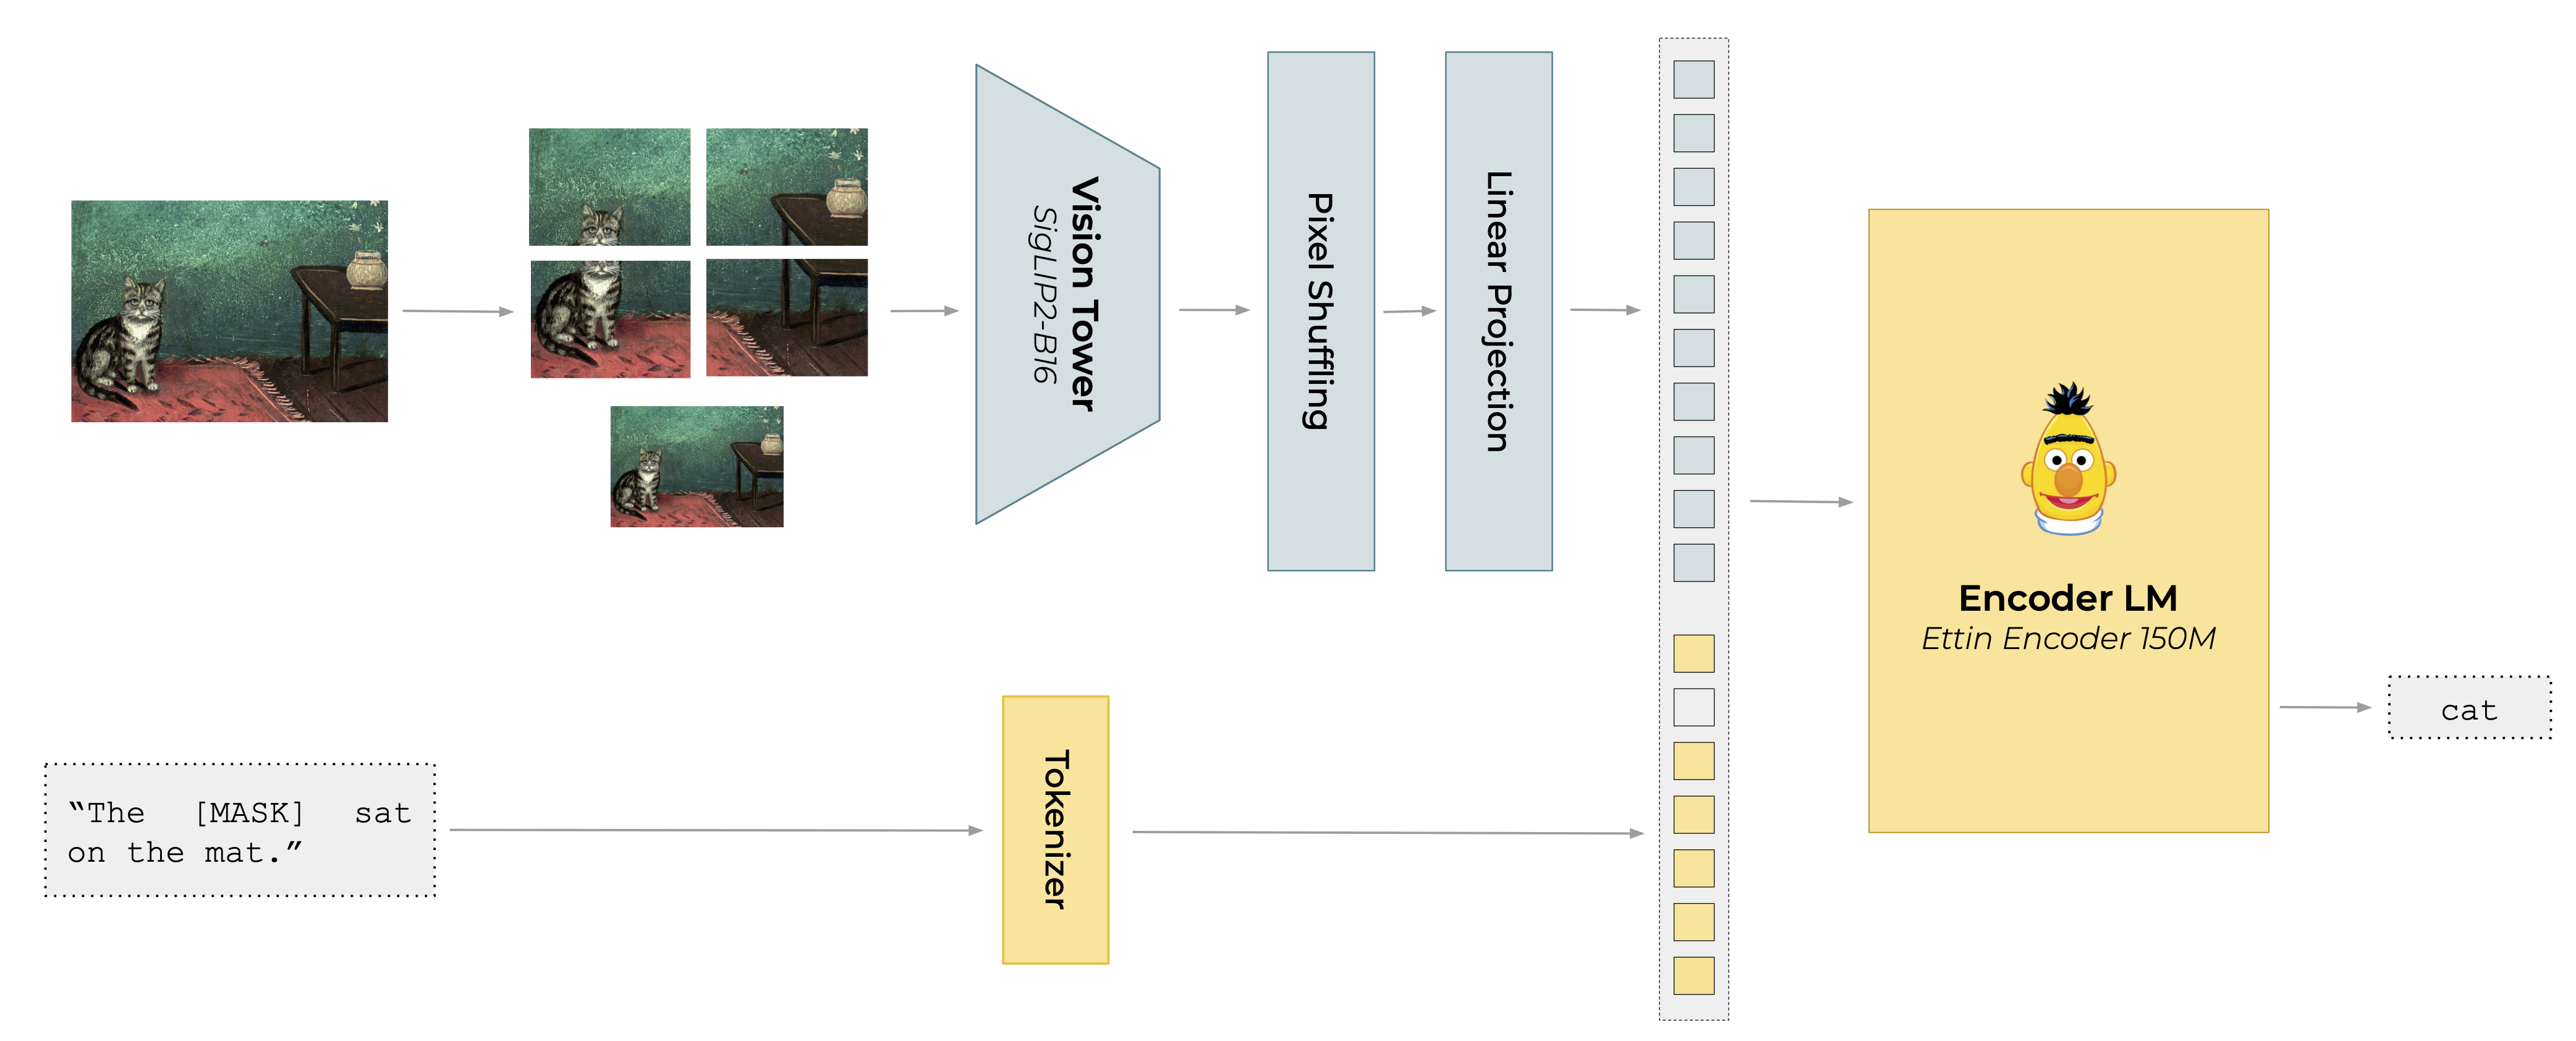
\includegraphics[width=0.99\textwidth]{images/modernvbert_figures/vbert_architecture.png}
    \caption[Early fusion architecture]{
    \textbf{MLM-based early fusion architecture.} The visual encoder produces patch representations, which are passed to a language model. 
    %We apply pixel shuffling to compress the visual representations produced by the vision tower.
    Our end-to-end bidirectional attention fused architecture is trained with Masked Language Modeling objectives and is perfectly suited for sequence and token-level representation tasks.}
    \label{fig:lf_architecture}
\end{figure}

\noindent\textbf{Model Architecture.}  
Our analysis are not centered around model architectures and to draw broadly applicable insights, we design vision-language models following current standard training practices.  In line with most recent work, we employ the early fusion architecture \sidecite{alayrac_flamingo_2022} illustrated in Figure~\ref{fig:lf_architecture}, in which visual patch embeddings produced by the vision encoder are projected into the language model input embedding space and concatenated with text token embeddings to encourage joint processing ~\sidecite{li2022blipbootstrappinglanguageimagepretraining, alayrac_flamingo_2022, wang2024qwen2vlenhancingvisionlanguagemodels, yang2025qwen251mtechnicalreport, marafioti2025smolvlmredefiningsmallefficient}. As described in \autoref{sec:modality-align}, we generalize the training loss to function both with causal and masked language modeling objectives.  
To handle dynamic resolutions, we split large images into 512$\times$512 pixel tiles as expected by the SigLIP encoder\sidenote{Images are downscaled (or upscaled) so that the lengths and widths reach a multiple of 512 pixels to preserve the aspect ratio, padding is used on the smaller side when necessary (i.e. a 1024x1000 px image would be padded to 1024x1024 px).}. Following current standard practices, we further process a downscaled version of the full image to improve inter-tile consistency and global visual understanding~\sidecite{lin2023sphinxjointmixingweights, ye2023ureaderuniversalocrfreevisuallysituated}. The vision tower produces 1024 pixel patch representations for each tile\sidenote{The SigLIP tower takes 512x512 px images and process them by 16x16 px patches \cite{dosovitskiy_image_2020}. This results in $(512/16)^2=1024$ patches.}, which we  compress to 64 tokens through \textit{pixel shuffling}~\sidecite{shi2016realtimesingleimagevideo} with a compression ratio $r=4$, following prior work on models of comparable size~\sidecite{marafioti2025smolvlmredefiningsmallefficient}. We highlight the impact of image resolution and this parameter on the number of visual tokens in Appendix~\ref{appendix:visual_tokens}.

% To handle dynamic resolutions, we split large images into 512$\times$512 pixel patches as expected by the SigLIP encoder, and further concatenate a downscaled version of the full image to improve inter-patch consistency and global visual understanding following current standard practices ~\sidecite{lin2023sphinxjointmixingweights, ye2023ureaderuniversalocrfreevisuallysituated}. To compress the information from sequences of large images, we apply pixel shuffling~\sidecite{shi2016realtimesingleimagevideo} with a ratio of $r=4$, following prior work on models of comparable size~\sidecite{marafioti2025smolvlmredefiningsmallefficient}.

% Note that we do not employ vision encoders with native resolution and RoPE-2D, as our focus is solely on single image representation learning using compact models. In this context, the additional computational overhead of such encoders is not justified.\paul{draft, I have to read qwen2vl carefully and understand the tradeoff more clearly}



% \noindent\textbf{Controlled Experimental Setup.}  
% We build on the publicly available checkpoints of \sidecite{gisserotboukhlef2025pretrainencodersmaskedlanguage}, which provide a fully controlled environment: all models share identical architectures, parameter counts, training datasets, and schedules, and differ only in the use of causal versus bidirectional attention masks. In addition, we include a decoder model from this work that has been annealed with MLM objectives, allowing us to evaluate whether decoders can effectively transition into encoder-like behavior. The full set of ablation models configurations is summarized in Table~\ref{tab:ablation_models}.

\noindent\textbf{Training Procedure.} Our experiments focus on retrieval performance. We employ a standard biphasic training procedure, in which we first run modality alignment to train a pretrained textual language model to understand visual inputs through language modeling objectives  ~\sidecite{liu_visual_2023} (\autoref{sec:modality-align}), then rely on a second text-image contrastive learning phase to learn efficient image representations ~\sidecite{radford_learning_2021} (\autoref{sec:contrastive_posttraining}). We further describe the general setup, and detail specific modifications to the default training procedure in the experiment section.

\subsection{Modality Alignment}
\label{sec:modality-align}
We align the vision encoder tower with the language model by training the image embedding projection layer to map visual features into the language model embedding space. The pretrained language model is also fine-tuned with Low-Rank Adapters (LoRA) \sidecite{hu_lora_2021}, allowing both image and text models to adapt jointly while reducing the risk of monomodal performance collapse \sidecite{alayrac_flamingo_2022, liu_visual_2023, laurencon_what_2024, mckinzie_mm1_2024, marafioti2025smolvlmredefiningsmallefficient}.

\noindent\textbf{Alignment Loss.} 
For decoder‑based models, we train with Causal Language Modeling (CLM) loss on the text tokens, as standardly done in VLM modality alignment:
\begin{equation}
\mathcal{L}_{\text{CLM}}
  = -\sum_{t=1}^{T} \log P_{\theta}\!\bigl(x_t \mid x_{<t}\bigr),
\end{equation}

where $x_{<t}$ denotes all tokens preceding position $t$. We generalize this training scheme to bidirectional encoders models, by using the Masked Language Modeling (MLM) loss on the textual tokens:
\begin{equation}
\mathcal{L}_{\text{MLM}}
  = -\sum_{t \in \mathcal{M}} \log P_{\theta}\!\bigl(x_t \mid x_{\backslash\mathcal{M}}\bigr),
\end{equation}
where $\mathcal{M}$ is the set of masked token positions and
$x_{\backslash\mathcal{M}}$ is the input with those tokens masked out.


\noindent\textbf{Modality Alignment Corpus.} Models are modality aligned on a large corpus in large parts derived from The Cauldron 2~\sidecite{laurencon_what_2024} and Docmatix~\sidecite{laurençon2024building}. Our objective being to train document focused retrieval models, we use an adjusted training mixture that upsamples images containing text and documents with varying level of complexities. Our final training corpus consists of approximately 2B text tokens, and includes diverse sources such as web pages, books, and scientific papers. Mixture details are given in Appendix~\ref{appendix:alignment_mixture}. We note that controlling the exact data distribution during this phase enables the models we train to specialize early and achieve good document focused downstream performances which many large models struggle with \sidecite{liu_improved_2023}.

\noindent\textbf{Parameters.} All models are trained using a masking ratio of 0.5 and user-prompt masking to avoid overfitting on chat-template format~\sidecite{huertaenochian2024instructionfinetuningdoesprompt, shi2024instructiontuninglossinstructions, allal2025smollm2smolgoesbig}. We employ WSD scheduler~\sidecite{hu2024minicpmunveilingpotentialsmall} with the first 5\% of the training as warmup, the last 20\% as decay and a maximum learning rate of 1e-4. The ablation models are aligned on 3.5B tokens. We provide additional details on the training setup in Appendix~\ref{appendix:implementation_details}.

\subsection{Contrastive Post-Training}
\label{sec:contrastive_posttraining}
Once the language model has learned to process image tokens jointly with text tokens, we specialize models through a contrastive post-training stage designed to enhance the semantic representation of the output embeddings produced by the model \sidecite{reimers2019sbert}. 

% We use a contrastive learning objective to modify the latent space of our base model to adapt it for similarity tasks. 

%We generate embeddings by mean pooling \maxou{cite paper backing this choice} token embeddings for encoder-based models, and by selecting the EOS token embeddings for decoder-based models \maxou{potentially here too? e.g. Qwen3-Embeddings}. 

\noindent\textbf{Post-training Pairs.} The post-training dataset used as starting point in our ablations comprises 118k document-query pairs from the ColPali corpus~\cite{faysse2025colpaliefficientdocumentretrieval} as well as another 118k of natural image-description pairs from the MSCOCO train set~\sidecite{lin_microsoft_2014}.

\textbf{Contrastive Loss.} We employ the InfoNCE loss~\sidecite{oord_representation_2018}, defined as

\begin{equation}
\mathcal{L}_{\text{InfoNCE}}(\mathbf{q},\mathbf{d^+})
  =-\log\frac{\Phi(\mathbf{q},\mathbf{d^+})}{\Phi(\mathbf{q},\mathbf{d^+}) + \sum_{\mathbf{d^-}\in\mathcal{N}_q}\Phi(\mathbf{q},\mathbf{d^-})},
\end{equation}

where $\mathbf{d^+}$ denotes the positive target for the query $\mathbf{q}$, $\mathcal{N}_\mathbf{q}=\mathcal{N}_\mathbf{q}^{\text{in}} \cup \mathcal{N}_\mathbf{q}^{\text{hard}}$ the set of negative targets (in-batch and hard negatives when mentioned), and $\Phi(\mathbf{q},\mathbf{d})$ a similarity function between the token(s) of the query and the documents.\sidenote{We use the last (EOS) token for causal models, and mean pool all sequence tokens for bidirectional encoders for single-vector models. Alternatively, we use all document and query tokens without pooling for late interaction matching \cite{faysse2025colpaliefficientdocumentretrieval}. Details in Appendix~\ref{appendix:similarity_functions}}. 
For general-domain post-training we compute the loss symmetrically~\sidecite{radford_learning_2021}.

\textbf{Batches Curation.} In contrastive learning, batch diversity critically impacts retrieval entropy. Overly heterogeneous batches lead to trivial retrievals, while curated batches yield richer training signals. We employ task-aware batching~\sidecite{li2023generaltextembeddingsmultistage}, grouping documents by source to ensure a homogeneous batch composition.


\subsection{Ablation Evaluation Setup}


The contrastively trained models are evaluated on retrieval and zero-shot classification tasks across multiple domains. Although the main focus remains document retrieval capabilities, evaluated by aggregating scores from the ViDoRe and ViDoRe v2\sidenote{\label{fn:vidorev2}We report only the English splits of ViDoRe v2, as our base models are trained on English data only.} \sidecite{macé2025vidorebenchmarkv2raising} benchmarks (nDCG@5), we also assess more generalist image retrieval capabilities by selecting tasks from MIEB~\sidecite{xiao2025miebmassiveimageembedding}. For natural image retrieval, we aggregate MSCOCO retrieval ~\sidecite{lin_microsoft_2014} and Flickr30k retrieval (nDCG@10) \sidecite{plummer_flickr30k_2015} test sets. Finally, following practices in \sidecite{muennighoff_mteb_2022}, we assess both zero-shot and fine-tuning abilities of our models on general classification tasks. Specifically, we measure classification accuracy by fine-tuning a logistic regression head on top of our model's embedding on Stanford Cars~\sidecite{6755945} and Food101~\sidecite{10.1007/978-3-319-10599-4_29}, and we evaluate zero-shot performance on FER2013~\sidecite{khaireddin2021facialemotionrecognitionstate} and EuroSAT~\sidecite{helber2019eurosatnoveldatasetdeep} and aggregate the results.


\section{What Makes a Great Visual Retriever?}

\begin{figure}[t] % <- 12 = approx. number of text lines to wrap
  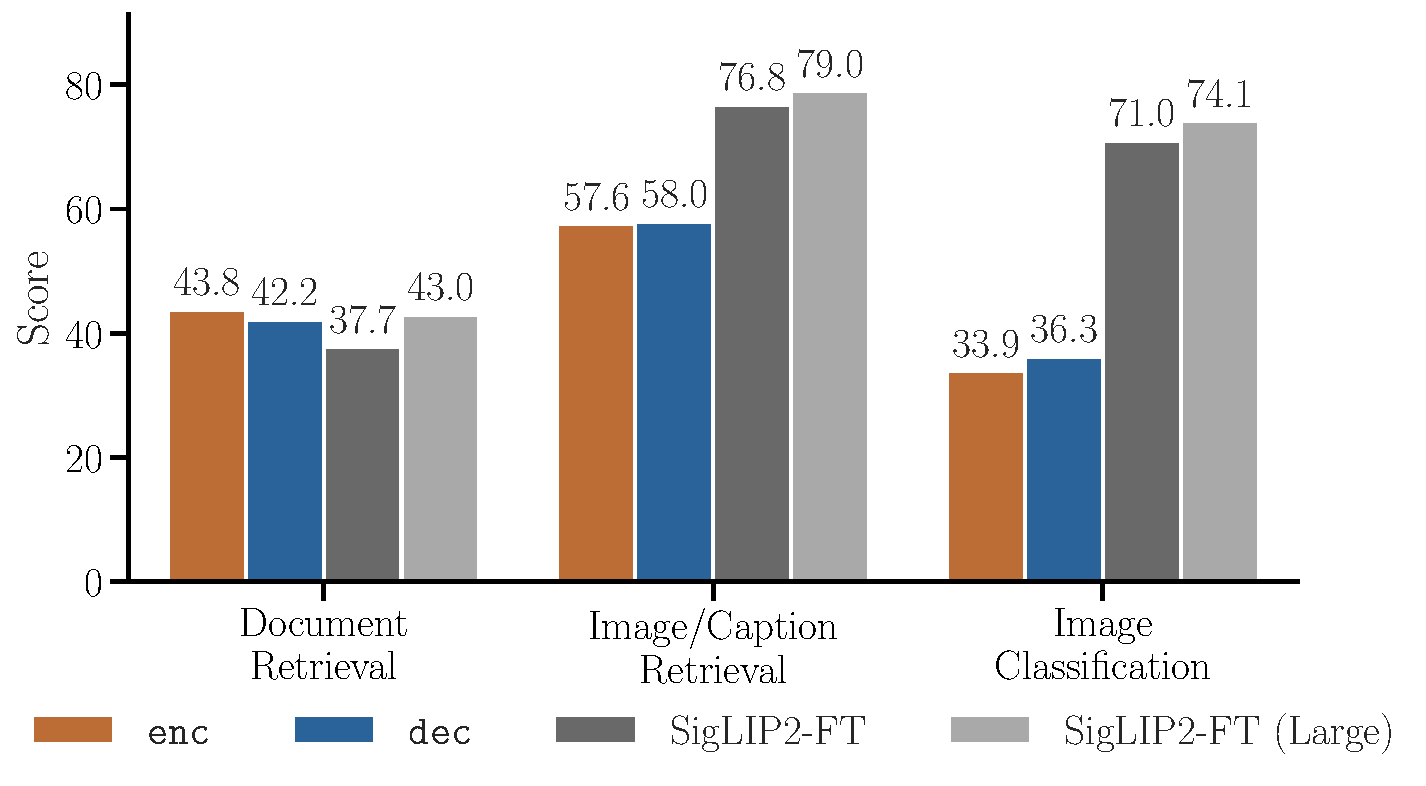
\includegraphics[width=0.95\linewidth]{images/modernvbert_figures/vbert_style/objective_downstream__rebuttal_ft.pdf}
    \caption[Modality alignment impact]{\textbf{Impact of Modality Alignment objective on downstream tasks.} Early Fusion of vision and text models boosts document retrieval tasks regardless of the LM objective, but degrades natural image and classification tasks w.r.t. the standalone \textit{fine-tuned} vision model SigLIP. Reported scores are aggregated MIEB scores (nDCG, Accuracy.)}
    \label{fig:objective_downstream}
\end{figure}


Vision-language retrievers built upon existing generative VLMs often inherit design choices and weights that may not be well suited for all embedding tasks. Here, we analyze these critical design choices hoping to derive clear insights for developing efficient visual retrievers. Importantly, although we assess design decisions at different stages of the training pipelines, evaluation are always done end-to-end on the final evaluation signal. 

%\anto{Suggestion for intro paragraph: Many vision-language retrieval systems adapt pre-trained generative models, but their weights are often not optimized for creating effective embeddings. In this section, we analyze the critical design choices in this adaptation process to provide clear guidelines for developing more efficient retrievers.}

\subsection{Modality Alignment Design}
\label{sec:ablation_tasks}

\noindent\textbf{Language modeling Modality Alignment improves document understanding.}
% According to benchmarks such as MIEB~\sidecite{xiao2025miebmassiveimageembedding}, dual encoder models trained explicitly on contrastive image-text tasks achieve superior performance in image classification tasks compared to VLMs. VLMs particularly excel at retrieving complex text-image relationships~\sidecite{jiang2024vlm2vectrainingvisionlanguagemodels}, yet, contrary to common belief, they do not enhance image representations themselves. In fact, they degrade performance in most natural image benchmarks. Instead, their strength lies in effectively aligning text and image tokens for zero-shot classification\paul{find work}. To substantiate this hypothesis, we designed experiments on document classification tasks, pooling image representations and applying classification heads. Results demonstrated that standalone image encoders possess sufficient capacity and information for these tasks, ultimately converging to similar performance levels regardless of the VLM training. This confirms that the critical contribution of VLMs lies in the modality alignment phase. For natural images, token-level alignment appears less critical, and the high-level features learned through large-scale contrastive training, as exemplified by SigLIP, are more impactful. Thus, contrastive training aligned with retrieval scenarios at inference is essential. \paul{What should we present here? Would results from @QM xp fit? Maybe we should focus on classification tasks here and stop reporting it later}
% On the other hand, these latest particularly excel at retrieving complex text-image relationships like documents-query ones~\sidecite{jiang2024vlm2vectrainingvisionlanguagemodels, chen2025mocamodalityawarecontinualpretraining}.
According to benchmarks such as MIEB~\sidecite{xiao2025miebmassiveimageembedding}, dual encoder models explicitly trained on contrastive image-text tasks outperform repurposed VLMs in natural image classification tasks. 
% We first study the impacts of aligning a pretrained Language Model (LM) with a vision tower through language modeling objectives, across different tasks.
%Using the checkpoints described in \autoref{sec:methodology}, 
To assess this, we train an encoder and a decoder vision-language model using the methodology described in \autoref{sec:methodology} on a mix of natural image and document data (alignment and contrastive training). We compare them with \textit{SigLIP2-FT}, the 378M dual vision encoder model whose vision component is used by the vision tower of both VLMs, and with the larger \textit{SigLIP2-FT Large} (881M parameters). Both SigLIP-FT models are finetuned in the same conditions as the VLMs, and initialized from pre-trained weights from scratch on billions of text-image pairs\sidenote{We report the performance of the untrained \textit{off-the-shelf} SigLIP in Appendix~\ref{appendix:objective_downstream}}.
As shown in Figure~\ref{fig:objective_downstream}, the two early fusion VLM variants severely underperform the SigLIP2-FT dual encoders on natural image tasks. In contrast, they achieve significant gains on document retrieval tasks (+6.1 nDCG@5 on ViDoRe and ViDoRe v2 datasets w.r.t. base), even edging out \textit{SigLIP2-FT Large} that contains 3.5x vision parameters more than both VLMs.

% This confirms high-level representation tasks do not benefit from the granular interactions between image and text tokens learned during the VLM modality alignment phase, but large-scale contrastive training remains superior. However, pairing a vision model with an LM enables token level interactions that create richer document understanding, aiding specific tasks even with less contrastive post-training.

This confirms large-scale contrastive training remains best for high-level image representation tasks (natural images), but sequentially combining a vision model with a pretrained language model facilitates document representation tasks, even with significantly less contrastive post-training. As the rest of this paper shows, steering away from the dual encoder architecture further enables improving performance through many avenues other than text to image contrastive training, for which supervised training samples can be hard to obtain.


% \begin{figure}
%     \centering
%     \includegraphics[width=0.9\linewidth]{images/modernvbert_figures/objective_downstream.png}
%     \caption{Impact of different objectives on downstream tasks. Aligning a language model with a vision tower through language modeling pretraining improves the performance of the model in document retrieval tasks. However, it degrades its performances in caption retrieval and classification tasks.}
%     \label{fig:objective_downstream}
% \end{figure}

% \noindent\textbf{Scaling the pretraining phase for better token representations.}  
% Prior work shows that scaling the pretraining phase of causal VLMs improves their generative abilities~\sidecite{beyer2024paligemmaversatile3bvlm, mckinzie_mm1_2024, wang2024qwen2vlenhancingvisionlanguagemodels}. We test whether similar gains hold in a bidirectional setting by evaluating checkpoints during pretraining with an MLM objective, up to 3.5B tokens. We compare this approach with the traditional CLM objective. Figure~\ref{fig:pt_scaling} presents the performance of the two training objectives across a diverse set of tasks. 
% The model improves across all tasks with additional pretraining data, showing the importance of scaling this phase. \textit{CLM offers an advantage in low-data regimes, but MLM seems to catches up and scales more effectively}. In document retrieval, MLM surpasses CLM.  
% % MLM scale better than CLM, especially in documental settings  
% % To counterbalance this plateau, we anneal the CLM-aligned decoder model using MLM to bring this objective scaling benefits. However, we observe a negative impact of such attention adaptation during cooldown. This might come from our model and scale, which may be too low to observe these gains.  
% % CLIP is the king in natural images  
% Image captioning and classification performances drop compared to the CLIP baseline vision tower. In contrast, the vision tower baseline is quickly outperformed in document retrieval. This finding suggests that \textit{token prediction pretraining yields embeddings better suited for document tasks than fully contrastively trained models}.  


% \begin{figure}[t]
%     \centering
%     \includegraphics[width=0.9\linewidth]{images/modernvbert_figures/pt_scaling.png}
%     \caption{Pretraining phase scaling. The dashed line marks the vision tower baseline. The orange curve shows the model initialized from a decoder LM with a \textit{CLM} objective, and the blue curve shows the model trained with an \textit{MLM} objective from an encoder LM. CLM performs better in low-data regimes, but MLM scales more effectively, surpassing CLM in document retrieval, while captioning and classification remain below the CLIP baseline.}
%     \label{fig:pt_scaling}
% \end{figure}


% \textit{Given that the initial training stage aims to align representations at the token level~\sidecite{jiang2024vlm2vectrainingvisionlanguagemodels}, we next evaluate whether MLM constitutes a more effective objective for learning multi-vector representations.}


\noindent\textbf{Scaling the modality alignment phase for better token representations.}  
Prior work shows that scaling the modality alignment phase of VLMs improves their generative abilities~\sidecite{beyer2024paligemmaversatile3bvlm, mckinzie_mm1_2024, wang2024qwen2vlenhancingvisionlanguagemodels}. We test whether similar gains hold in retrieval by contrastively fine-tuning \texttt{enc} checkpoints during MLM modality alignment. Figure~\ref{fig:pt_scaling} illustrates the results of post-trained checkpoints on diverse tasks. 
Although document retrieval improves consistently with more modality alignment data -- largely surpassing the vision tower evaluated in isolation and showing clear scaling benefits -- natural image tasks plateau past 1B tokens, far from the standalone dual encoder baseline. This shows that document and natural image retrieval leverage different mechanisms and should not be optimized the same way. \textit{Document Retrieval benefits from learning fine-grained interactions between image and text tokens through the language model, while the LM has limited utility for high level natural image tasks}.


\begin{figure}[t]
    \centering    
    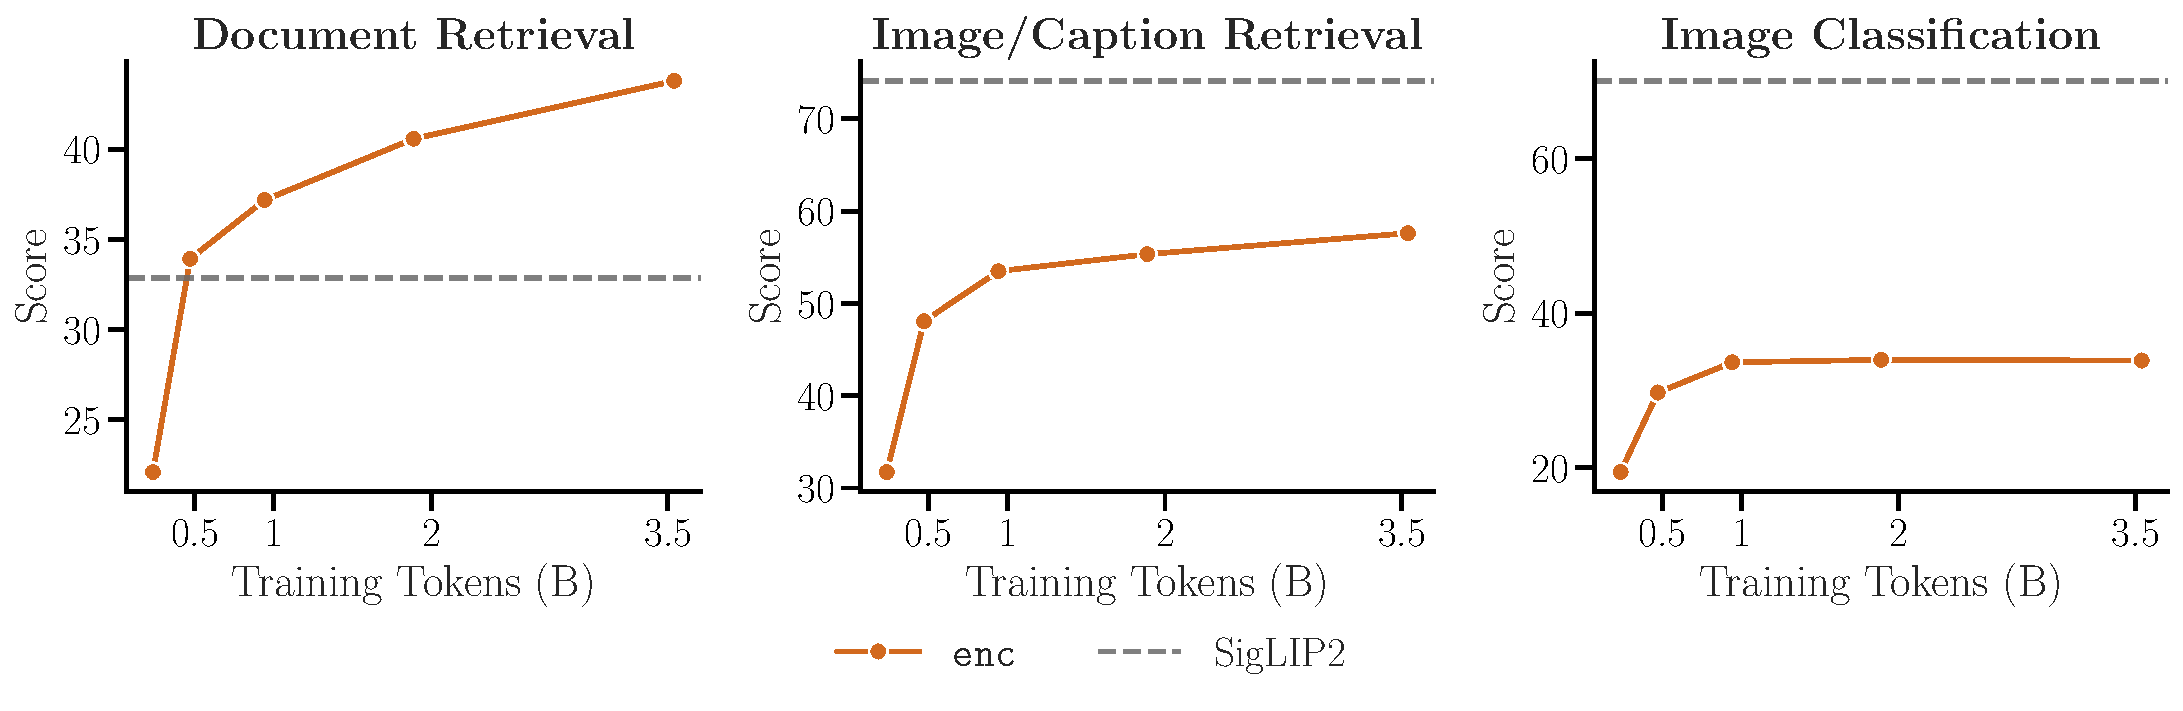
\includegraphics[width=0.95\textwidth]{images/modernvbert_figures/vbert_style/pt_scaling.pdf}
    \caption[Modality alignment scaling]{\textbf{Modality alignment scaling of early fusion encoders for up to 1 epoch (3.5B tokens) of data.} The dashed line indicates the vision encoder evaluated standalone without further training. Our findings show that retrieval tasks benefits from extended modality alignment phase, particularly in document retrieval, where performance quickly surpasses that of the standalone vision encoder. }
    % \manu{paul: could we have this in terms of B tokens seen instrad of steps ? remove average, increase fonts}}
    \label{fig:pt_scaling}
\end{figure}


\noindent\textbf{Bidirectional attention fully unlocks Late Interaction.}
Inspired by the effectiveness of bidirectional attention in text-only retrieval~\sidecite{gisserotboukhlef2025pretrainencodersmaskedlanguage, weller2025seqvsseqopen}\sidenote{\cite{chen2025mocamodalityawarecontinualpretraining} investigate post-hoc removal of the attention mask during visual retrieval fine-tuning.}, we investigate if it surpasses causal attention in \textit{visual document retrieval}, particularly when using the multi-vector late interaction matching common in SOTA visual retrievers~\sidecite{khattab2020colbert, faysse2025colpaliefficientdocumentretrieval}.
% Table~\ref{table:vidore_alignment_objective} presents the results on the ViDoRe benchmark suite when training a visual retriever with different attention masking and objective loss.  
Figure~\ref{fig:enc_dec_multivec} reports single vector and late interaction results on the ViDoRe benchmark for various model variants. On top of the standard \texttt{enc} (MLM) and \texttt{dec} (CLM) models, we evaluate the \texttt{dec-enc} and the  \texttt{dec} models modality aligned with MLM objectives to determine whether bidirectional attention capabilities can be obtained in later stages of training.

Single-vector embedding results are close between bidirectional and causal attention models for document retrieval, with \texttt{enc} slightly outperforming \texttt{dec} by +1.6 nDCG@5. 
% Single-vector embedding results are close between bidirectional and causal attention models, with \texttt{dec} slightly outperforming \texttt{enc}. 

Intuitively however, bidirectional attention makes a huge difference when used in late interaction settings, substantially exceeding the causal counterpart by +10.6 nDCG@5. 
% \paul{@MF recheck jai du changer car dec est legerement meilleur en single vec - ouais true que en doc}
Causal decoders are incapable of correctly contextualizing image or text token representations seen at the beginning of the sequences. \textit{This is a key result as almost all current visual retrievers, including late interaction variants, are causal models, clearly indicating some performance is left on the table.}

Removing the causal attention mask during training does not suffice to recover the \texttt{enc} late interaction performance at these data regimes. This indicates converting trained decoders as late interaction retrievers is highly non trivial, and confirms the insights from \sidecite{weller2025seqvsseqopen}; when possible, training encoder models from scratch remain better for retrieval tasks.



% \begin{table*}[ht]
%   \centering
%   \renewcommand{\arraystretch}{1.2}
%   \small
%   \resizebox{0.6\textwidth}{!}{%
%   \begin{tabular}{@{} >{}l cc >{\columncolor{avgcol}}c}
%     % Group banners with distinct colors, no top rule
    
%     % & \multicolumn{2}{>{\columncolor{grpA}}c}{\textbf{Doc. Retrieving}}  \\
%     % \cmidrule(lr){2-3}
%     & \rot{ViDoRe(v1)} & \rot{ViDoRe(v2)} 
%     & \rot{\textbf{Average}} \\
%     \midrule
%     \multicolumn{3}{@{}l}{\itshape Causal Base LM}\\
%     CLM Alignment & 67.1 & 41.4 & 54.3 \\
%     MLM Alignment & 65.6 & 35.1 & 50.4 \\
%     \hspace{3pt} + \textit{Base Model Annealing} & 67.4 & 38.9 & 53.1 \\
%     \midrule
%     \multicolumn{3}{@{}l}{\itshape Bidirectional Base LM}\\
%     MLM Alignment & \textbf{79.1} & \textbf{50.6} & \textbf{64.9}  \\
%     \bottomrule
%   \end{tabular}%
%   }
%   \caption{Scores (nDCG@5) of the models on ViDoRe v1 and ViDoRe v2 \textit{english} splits\footnote{Our base LM models are trained on english only, thus evaluating on multilingual splits for such comparison would be mostly noise.} when training a visual retriever with different attention masking and objective loss. \textit{Causal Base LM}  are the models based on a decoder LM, while \textit{Bidirectional Base LM} are the one from an encoder LM. \textit{Base Model Annealing} is the LM backbone annealed as an encoder \textbf{before modality alignment}.}
%   \label{table:vidore_alignment_objective}
% \end{table*}

% \textit{For a fixed model, image resolution is an important factor influencing downstream performance. We therefore examine how resolution impacts embedding tasks, and whether its effect varies by task type.}

\begin{figure*}[t]
    \centering

    \includegraphics[width=0.43\textwidth]{images/modernvbert_figures/enc_dec_vidore_palette.pdf}
    \caption[Attention mask impact]{\textbf{Impact of attention masks and training objectives on document retrieval performances.} 
    We report the average nDCG@5 on English splits of ViDoRe benchmarks for models post-trained on ColPali.
    % Employing native bidirectional attention outperforms the other approaches when used in multi-vector settings 
    }
    \label{fig:enc_dec_multivec}

\end{figure*}

\begin{figure*}[t]
    \centering

    \renewcommand{\arraystretch}{1.1}
    \small
    \resizebox{0.48\textwidth}{!}{%
    \begin{tabular}{@{} l c ccc >{\columncolor{avgcol}}c}
    & {HR Cooldown} & \rot{Document Retrieval} & \rot{Image/Caption Retrieval} & \rot{Image Classification} & \rot{\textbf{Average}} \\

    \midrule
    512px  & \xmark & 30.7 & \underline{58.8} & \textbf{41.4} & 43.6 \\
    1024px & \xmark & 42.2 & \textbf{58.9} & \underline{37.2} & \textbf{46.1} \\
    2048px & \xmark & \underline{43.8} & 57.6 & 33.9 & 45.1 \\
    2048px & \cmark & \textbf{45.8} & 57.8 & 33.7 & \underline{45.8} \\

    \bottomrule
    \end{tabular}%
    }
    \caption[Image resolution effect]{\textbf{Effect of image resolution on VL encoder abilities.} Document retrieval performance increases with higher image resolution. Further annealing the encoder on high-resolution images (HR Cooldown) at the end of modality alignment yields additional gains. By contrast, for non-document tasks, raising the resolution tends to degrade performance.}
    \label{table:image_resolution}

\end{figure*}

% \begin{figure*}[t]
%     \centering
%     % Left side: first figure (single subfigure kept)
%     \begin{minipage}{0.48\textwidth}
%         \centering
%         \includegraphics[width=0.9\textwidth]{images/modernvbert_figures/enc_dec_vidore_palette.pdf}
%         \caption{\textbf{Impact of attention masks and training objectives on document retrieval performances.} 
%         We report the average nDCG@5 on English splits of ViDoRe benchmarks for models post-trained on ColPali.
%         % Employing native bidirectional attention outperforms the other approaches when used in multi-vector settings 
%         } 
%         \label{fig:enc_dec_multivec}
%     \end{minipage}%
%     \hfill
%     % Right side: second figure + table
%     \begin{minipage}{0.48\textwidth}
%         \renewcommand{\arraystretch}{1.1}
%         \small
%         \resizebox{\textwidth}{!}{%
%         \begin{tabular}{@{} l c ccc >{\columncolor{avgcol}}c}
%         & {HR Cooldown} & \rot{Document Retrieval} & \rot{Image/Caption Retrieval} & \rot{Image Classification} & \rot{\textbf{Average}} \\
    
%         \midrule
%         512px & \xmark & 30.7 & \underline{58.8} & \textbf{41.4} & 43.6 \\
%         1024px & \xmark & 42.2 & \textbf{58.9} & \underline{37.2} & \textbf{46.1} \\
%         2048px & \xmark & \underline{43.8} & 57.6 & 33.9 & 45.1 \\
%         2048px & \cmark & \textbf{45.8} & 57.8 & 33.7 & \underline{45.8} \\
        
%         \bottomrule
%         \end{tabular}%
%         }
%         \captionof{table}{\textbf{Effect of image resolution on VL encoder abilities.} Document retrieval performance increases with higher image resolution. Further annealing the encoder on high-resolution images (HR Cooldown) at the end of modality alignment yields additional gains. By contrast, for non-document tasks, raising the resolution tends to degrade performance.}
%         \label{table:image_resolution}
            
%         % \vspace{1em}
%         % \centering        \includegraphics[width=0.9\linewidth]{images/modernvbert_figures/pt_scaling.png}
%         % \captionof{figure}{\textbf{Pretraining phase scaling.} The dashed line marks the vision tower baseline. \paul{TODO: I wait to fix what tiles we show here before writting the caption(mean of tasks per domain like above, or per task)}}
%         % \label{fig:pt_scaling}
%     \end{minipage}
% \end{figure*}


% However, we also observe a negative correlation with performance on tasks that involve natural images. This suggests that the multiple high-resolution crops generated during preprocessing may obscure global separable features necessary for classification, and that passing one image in the size expected by the vision tower is optimal. 
%These results highlight the importance of flexible, resolution-aware preprocessing pipelines that can adapt hierarchically to the native resolution of each input image.

% \begin{table*}[t]
%   \centering
%   \renewcommand{\arraystretch}{1.2}
%   \small
%   \resizebox{0.5\textwidth}{!}{%
%   \begin{tabular}{@{} l c ccc >{\columncolor{avgcol}}c}
%     & {HR Cooldown} & \rot{Document Retrieval} & \rot{Caption Retrieval} & \rot{Zero-Shot Classification} & \rot{\textbf{Average}} \\

%     \midrule
%     512px & \xmark & 30.7 & 58.8 & 45.1 & 44.9 \\
%     1024px & \xmark & 42.2 & \textbf{58.9} & 42.8 & \textbf{48.0} \\
%     2048px & \xmark & 43.8 & 57.6 & 40.4 & 47.3 \\
%     2048px & \cmark & \textbf{45.8} & 57.8 & 39.2 & 47.6 \\
    
%     \bottomrule
%   \end{tabular}%
%   }
%   \caption{\textbf{Effect of image resolution on VL encoder abilities.} Document retrieval performance increases with higher image resolution. Further annealing the encoder on high-resolution images (HR Cooldown) during pretraining yields additional gains. By contrast, for non-document tasks, raising the resolution tends to degrade performance.}
%   \label{table:image_resolution}
% \end{table*}

% \begin{table*}[t]
%   \centering
%   \renewcommand{\arraystretch}{1.1}
%   \small
%   \resizebox{\textwidth}{!}{%
%   \begin{tabular}{@{} l cc ccc >{\columncolor{avgcol}}c}
%     & {HR Cooldown} & {Resize at Inference} & \rot{Document Retrieval} & \rot{Caption Retrieval} & \rot{Zero-Shot Classification} & \rot{\textbf{Average}} \\

%     \midrule
%     512px & \xmark & \cmark & 30.7 & 58.8 & 45.1 & 44.9 \\
%     1024px & \xmark & \cmark & 42.2 & \textbf{58.9} & 42.8 & 48.0 \\
%     2048px & \xmark & \cmark & 43.8 & 57.6 & 40.4 & 47.3 \\
%     2048px & \cmark & \cmark & \textbf{45.8} & 57.8 & 39.2 & 47.6 \\
%     2048px & \xmark & \xmark & 42.6 & 56.0 & \textbf{46.7} & \textbf{48.5} \\
    
%     \bottomrule
%   \end{tabular}%
%   }
%   \caption{\textbf{Effect of image resolution on VL encoder abilities.} Document retrieval performance increases with higher image resolution. Further annealing the encoder on high-resolution images (HR Cooldown) during pretraining yields additional gains. By contrast, for non-document tasks, raising the resolution tends to degrade performance, with best average score achieved when not resizing the input images during inference.}
%   \label{table:image_resolution}
% \end{table*}

\subsection{Contrastive Training Design} 

The previous subsection established bidirectional encoder models to often be the best option when training visual retrievers. In the following experiments, we assess contrastive training choices and only report results for the encoder model for simplicity.

% After the first stage, the model can perform token prediction, but its latent space is not optimized for general concept embeddings. A common solution is to add a second stage with a contrastive objective~\sidecite{jiang2024vlm2vectrainingvisionlanguagemodels, jiang2024e5vuniversalembeddingsmultimodal, chen2025mme5improvingmultimodalmultilingual, chen2025mocamodalityawarecontinualpretraining}.  
% This stage aligns concept representations across modalities at the sentence level, yielding models well suited for zero-shot tasks~\sidecite{radford_learning_2021, zhai_sigmoid_2023}.  
% \paul{Un truc style on a vu avant que token-level c'est bien pour documentaire masi CL aide sur le reste. On regarde comment on peut scale notre dataset pour tirer un max de perf across all tasks} In this section, we search for the most effective contrastive post-training mix to draw maximum capabilities. 

% \textit{While additional paired data are required to close the performance gap on natural image tasks, such resources remain limited. This raises the question of how alternative data sources might be leveraged to address this gap.}


\noindent\textbf{Image resolution benefits are task-specific.} 
Image resolution plays a critical role in VLM generative capabilities, notably in document-focused tasks, as higher-resolution inputs enables the model to capture finer visual cues~\sidecite{hu2024mplugdocowl2highresolutioncompressingocrfree, marafioti2025smolvlmredefiningsmallefficient}.
%We examine how these resolution dynamics transfer to embedding tasks. 
Modality alignment is done at a fixed image resolution of 1024 pixels (longer side) and we report scores of contrastive training runs with varying settings in Table~\ref{table:image_resolution}. To vary the resolution, images of the highest quality available are scaled to the desired size (often downscaled) before being fed to the image tokenizer. Our findings confirm that embedding tasks are strongly sensitive to image-resolution. In particular, \textit{training with higher resolution inputs substantially improves the results on visual document retrieval benchmarks}, consistent with prior work in generative settings~\cite{beyer2024paligemmaversatile3bvlm, mckinzie_mm1_2024}. Furthermore, adding a cool-down phase by showing higher-resolution images towards the end of the modality alignment phase yields additional gains. This suggests that models can adapt their attention mechanisms to finer details when exposed to increased resolution. Interestingly, these findings do not hold in natural image tasks, where high resolution can even degrade performance.


% \noindent\textbf{Scaling the modality alignment phase for better token representations.}  
% Prior work shows that scaling the CLM modality alignment phase of VLMs improves their generative abilities~\sidecite{beyer2024paligemmaversatile3bvlm, mckinzie_mm1_2024, wang2024qwen2vlenhancingvisionlanguagemodels}. We test whether similar gains hold in a retrieval setting by evaluating checkpoints during modality alignment with an MLM objective, for up to 3.5B tokens. Figure~\ref{fig:pt_scaling} illustrates the results of the post-trained checkpoints on diverse tasks. 
% The model consistently improves across all retrieval tasks with an increasing amount of alignment data. This is similar to what is observed for generative tasks, suggesting that the model learns to create richer token representations with the information available in the images during this modality alignment stage.

% \begin{figure}[t]
%     \centering    \includegraphics[width=0.95\textwidth]{images/modernvbert_figures/pt_scaling.png}
%     \caption{\textbf{Modality alignment scaling.} The dashed line marks the vision tower baseline. \paul{TODO: I wait to fix what tiles we show here before writing the caption(mean of tasks per domain like above, or per task)}}
    
%     \label{fig:pt_scaling}
% \end{figure}

% \begin{figure}[t]
%     \centering    \includegraphics[width=0.85\textwidth]{images/modernvbert_figures/finegrain/pt_scaling.png}
%     \caption{Pretraining phase scaling. The dashed
% line marks the vision tower baseline. \paul{TODO: I wait to fix what tiles we show here before writing the caption(mean of tasks per domain like above, or per task)}}
    
%     \label{fig:pt_scaling_finegrain}
% \end{figure}

% \begin{table*}[b]
%   \centering
%   \renewcommand{\arraystretch}{1.2}
%   \small
%   \resizebox{\textwidth}{!}{%
%   \begin{tabular}{@{} >{}l c c c >{\columncolor{avgcol}}c}
%     & {Document Retrieval} & {Caption Retrieval} & {Zero-Shot Classification} & {\textbf{Average}} \\

%     \midrule
%     Baseline CL Mix & 43.9 & \textbf{57.2} & 40.6 & 47.2 \\
%     + \textit{Text$\rightarrow$Text Pairs} & 45.6 & 53.2 & 42.3 & 47.0 \\
%     + \textit{Image$\rightarrow$Caption Pairs} & \textbf{45.8} & 54.4 & \textbf{44.4} & \textbf{48.2} \\
    
%     \bottomrule
%   \end{tabular}%
%   }
%   \caption{\textbf{Impact of contrastive post-training mixtures on downstream tasks.} Incorporating text-only pairs improves performance on document retrieval, but degrades other performances. Adding natural images-captions pairs substantially enhances performance on zero-shot classification tasks.}
%   \label{table:cl_mix_impact}
% \end{table*}

\begin{table*}[b]
  \centering
  \renewcommand{\arraystretch}{1.4}
  \small
  \resizebox{\textwidth}{!}{%
  \begin{tabular}{@{} >{}l  ccc >{\columncolor{avgcol}}c}
    & {Document Retrieval} & {Image/Caption Retrieval} & {Image Classification} & {\textbf{Average}} \\

    \midrule
    Baseline CL Mix & 43.9 & \textbf{57.2} & 36.1 & 45.7 \\
    + \textit{Text$\rightarrow$Text Pairs} & 45.6 & 53.2 & 35.7 & 44.8 \\
    + \textit{Image$\rightarrow$Caption Pairs} & \textbf{45.8} & 54.4 & \textbf{49.9} & \textbf{50.0} \\
    
    \bottomrule
  \end{tabular}%
  }
  \caption[Contrastive training mixtures impact]{\textbf{Impact of contrastive training mixtures on downstream tasks.} Incorporating text-only pairs improves performance on document retrieval, but degrades other performances. Adding natural images-captions pairs substantially enhances performance on classification tasks.}
  \label{table:cl_mix_impact}
\end{table*}


\noindent\textbf{Increasing the pool of contrastive pairs.}
\label{sec:scaling=-cont}
% \quentin{A series of ablation studies on our post-training data composition revealed two key insights. First, incorporating unimodal text-only pairs from \cite{thakur2025rlhn} markedly enhances performance on visual document retrieval \ref{table:cl_mix_impact}. We attribute this enhancement to the model learning a more complex semantic understanding from the textual data, which successfully transfers across modalities to the image-text task. Second, we found that adding the \natcap{} dataset is crucial for preserving the model's general vision capabilities. By expanding the contrastive dataset and increasing the variety of image types, it effectively counteracts the performance degradation on image classification benchmarks typically seen when aligning the original SigLIP baseline with our text encoder.}
A severe limitation that current visual retrievers face is the lack of large volumes of high quality (document image, query pairs). 
Previous work \sidecite{ma2024unifyingmultimodalretrievaldocument, faysse2025colpaliefficientdocumentretrieval, jiang2024vlm2vectrainingvisionlanguagemodels, zhang2025gmeimprovinguniversalmultimodal} has relied on a mix of repurposed existing visual question answering datasets and synthetically generated queries with external LLMs. Even put together however, the field is only a year old, and these datasets remain small in size and often of poor quality.


% As described in Section ~\ref{sec:ablation_tasks}, using modality alignment is only one phase of training stage reduces performance in natural image tasks compared to the vision tower backbone. This underscores the need for extensive contrastive post-training to obtain stronger single-vector representations~\sidecite{radford_learning_2021}. 
% \paul{on peut affiner la motiv}
% However, the absence of large-scale and high-quality multimodal contrastive datasets constrains the scalability of this phase. To address this, we investigate whether incorporating additional data sources incrementally can mitigate these limitations. 
A central question in our study is whether the abundance of \emph{text-only} query–document pairs can be exploited to improve \emph{visual} retrieval via cross-modal capability transfer. To probe this, we run contrastive training under three regimes. Unlike prior work that “warms up” visual retrievers or trains exclusively with text-only pairs \sidecite{ma2024unifyingmultimodalretrievaldocument, jiang2024e5vuniversalembeddingsmultimodal}, we \emph{interleave} text-only pairs and text–image pairs throughout training at a 1:1 ratio. The dataset sources are detailed in Appendix~\ref{appendix:contrastive_mix}

As reported in Table~\ref{table:cl_mix_impact}, incorporating text-only pairs yields a sizeable improvement on visual document retrieval (+1.7 \textsc{nDCG}@5), indicating clear cross-modal transfer—likely facilitated by the backbone’s jointly learned text–image embedding space. This result suggests that domain-specific training corpora can be assembled irrespective of native modality, reducing duplication of effort and lowering data-collection costs.

We further evaluate training with \natcap{}, a corpus of natural images paired with synthetic, highly detailed captions (see Appendix~\ref{appendix:natcap}). This scaling step improves downstream performance across the board—most notably on natural-image tasks, and with a smaller but consistent gain on document retrieval (+0.2 \textsc{nDCG}@5). Together, these findings underscore the importance of scaling contrastive learning with high-quality data, but which doesn't need to be exclusively image document focused.


% \begin{table*}[t]
%   \centering
%   \renewcommand{\arraystretch}{1.2}
%   \small
%   \resizebox{\textwidth}{!}{%
%   \begin{tabular}{@{} >{}l cccc >{\columncolor{avgcol}}c}

%     & Document Retrieval & Captioning & Classification (0S) & Classification (LP)
%     & \textbf{Average} \\

%     \toprule
%     % \multicolumn{6}{@{}l}{\itshape Single-Vector} \\
%     % ColPali & -- & -- & -- & -- & -- \\
%     % \hspace{3pt} + \textit{MSCOCO} & 43.9 & \textbf{57.2} & 19.8 & 52.2 & 43.3 \\
%     Baseline CL mix & 43.9 & \textbf{57.2} & 19.8 & 52.2 & 43.3 \\
%     \hspace{3pt} + \textit{\natcap{}} & \underline{44.9} & 53.7 & \underline{36.2} & \underline{59.8} & 48.7 \\
%     \hspace{3pt} + \textit{Text$\rightarrow$Text Data}& \textbf{45.8} & \underline{54.4} & \textbf{39.8} & \textbf{60.0} & \textbf{50.0} \\
%     % \midrule
%     % \multicolumn{6}{@{}l}{\itshape Multi-Vector} \\
%   \end{tabular}%
%   }
%   \caption{Impact of contrastive post-training mixtures on downstream tasks. Adding \natcap{} substantially enhances performance on image classification tasks, but leads to a decrease in performance on natural image captioning. Incorporating unimodal text data improves performance on document retrieval  and zero-shot tasks.}
%   \label{table:cl_mix_impact}
% \end{table*}

% \begin{table*}[h]
%   \centering
%   \renewcommand{\arraystretch}{1.2}
%   \small
%   \resizebox{\textwidth}{!}{%
%   \begin{tabular}{@{} >{}l ccc >{\columncolor{avgcol}}c}

%     & \rot{Document Retrieval} & \rot{Caption Retrieval} & \rot{Zero-Shot Classification}
%     & \rot{\textbf{Average}} \\

%     \toprule
%     % \multicolumn{6}{@{}l}{\itshape Single-Vector} \\
%     % ColPali & -- & -- & -- & -- & -- \\
%     % \hspace{3pt} + \textit{MSCOCO} & 43.9 & \textbf{57.2} & 19.8 & 52.2 & 43.3 \\
%     Baseline CL mix & 43.9 & \textbf{57.2} & \underline{19.8} & \underline{40.3} \\
%     \hspace{3pt} + \textit{Text$\rightarrow$Text Pairs (RLHN)}& \underline{45.6} & 53.2 & 18.2 & 39.0 \\
%     % \hspace{3pt} + \textit{\natcap{}} & \underline{44.9} & 53.7 & \underline{36.2} & 44.9 \\
%     \hspace{3pt} + \textit{Image$\rightarrow$Caption Pairs (\natcap{})} & \textbf{45.8} & \underline{54.4} & \textbf{39.8} & \textbf{46.7} \\
%     % \midrule
%     % \multicolumn{6}{@{}l}{\itshape Multi-Vector} \\
%     \bottomrule
%   \end{tabular}%
%   }
%   \caption{\textbf{Impact of contrastive post-training mixtures on downstream tasks.} Incorporating unimodal text data improves performance on document retrieval, but degrades other performances. Adding \natcap{} substantially enhances performance on zero-shot classification tasks.}
%   \label{table:cl_mix_impact}
% \end{table*}



% \noindent\textbf{Merging Models.} 

% \begin{table*}[t]
%   \centering
%   \renewcommand{\arraystretch}{1.2} % Adjusts row spacing for better readability
%   \small % Use a smaller font size for the table
%   % Resize the table to fit the width of the text area
%   \resizebox{\textwidth}{!}{%
%   \begin{tabular}{@{} l l c cc cc c @{}} % Column formatting
%     % --- Column Headers with Grouping and Colors ---
%     &
%     & \multicolumn{1}{>{\columncolor{grpA}}c}{\textbf{Captioning}}
%     & \multicolumn{2}{>{\columncolor{grpB}}c}{\textbf{Doc. Retrieval}}
%     & \multicolumn{2}{>{\columncolor{grpC}}c}{\textbf{Natural Image}}
%     & \multicolumn{1}{>{\columncolor{grpD}}c}{\textbf{Other}} \\
    
%     % Use cmidrule for partial lines under the main groups
%     \cmidrule(lr){3-3} \cmidrule(lr){4-5} \cmidrule(lr){6-7} \cmidrule(lr){8-8}
    
%     % --- Sub-headers for specific datasets/tasks ---
%     Task & Model & Image Captioning & ViDoRe(v1) & ViDoRe(v2) & MSCOCO & Flickr30k & Others \\
%     \midrule
    
%     % --- Table Data ---
%     % Using \texttt{} for model names to correctly display underscores and improve readability
%     4 & \texttt{baseline\_x\_baseline-\natcap{}-text-2\_t075} & 0.576 & 0.484 & 0.136 & 0.478 & 0.674 & 0.898 \\
%     0 & \texttt{baseline\_x\_baseline-\natcap{}-text-05}     & 0.561 & 0.483 & 0.138 & 0.466 & 0.656 & 0.901 \\
%     1 & \texttt{baseline\_x\_baseline-\natcap{}-text-2}      & 0.561 & 0.480 & 0.132 & 0.467 & 0.655 & 0.900 \\
%     5 & \texttt{baseline\_x\_baseline-text-07\_x\_...-\natcap{}} & 0.544 & 0.469 & 0.125 & 0.451 & 0.637 & 0.901 \\
%     2 & \texttt{baseline\_x\_baseline-\natcap{}-text-2\_avg}  & 0.551 & 0.462 & 0.129 & 0.450 & 0.653 & 0.898 \\
%     3 & \texttt{baseline\_x\_baseline-\natcap{}-text-2\_t025} & 0.537 & 0.466 & 0.127 & 0.446 & 0.628 & 0.900 \\
%     \bottomrule
%   \end{tabular}%
%   }
%   \caption{Performance comparison of different model configurations across a variety of downstream tasks. The table evaluates performance on image captioning, document retrieval (ViDoRe), natural image tasks (MSCOCO, Flickr30k), and other benchmarks.}
%   \label{table:model_performance_comparison}
% \end{table*}

\section{Building a Small yet Mighty Visual Retriever.}
% \noindent\textbf{Assymetric encoders.} 
% \noindent\textbf{Ensembled embeddings.} 

% \manu{Maybe we can take the kaobox takeaway style a bit similar to here ? \url{https://arxiv.org/pdf/2410.10781}}
% \noindent\textbf{Selecting the right recipe.} Putting together the results from our experiment, we devise a training recipe for a small visual document retriever. 

% Our ablation studies yields key insights on training early fusion visual encoders. 
% Notably, practitioners should select architectures according to task needs: fused VLMs are preferable for document tasks due to their ability to generate token-level representations, whereas lightweight CLIP-style ViTs offer superior sentence-level alignment particularly useful in image captioning and classification. When building visual document retrievers from scratch, practitioners should prioritize bidirectional attention to fully exploit the benefits of a token-level alignment with late interaction.
% When starting from pretrained models and larger parameter scales, we suggest annealing causal VLMs into bi-directional encoders using methods such as MoCa~\sidecite{chen2025mocamodalityawarecontinualpretraining}. This strategy combines the advantages of bi-directional attention in late interaction with the rich semantic and world knowledge captured during large-scale causal pretraining.

% \paul{Linking stuff: We want to build a visual document retriever from scratch, freeing ourselves from the constraint of repurposing a VLM. Building on our insights, [...].}

\subsection{Training.} 

\noindent\textbf{Recipe.} Putting together the results from our experiments, we devise a training recipe for a small visual document retriever \flagship{}. It combines a state-of-the-art 150M text bidirectional encoder~\sidecite{weller2025seqvsseqopen} with the ModernBERT architecture \sidecite{modernbert} and a small vision encoder SigLIP2-16B-512 of 100M parameters~\sidecite{tschannen2025siglip2multilingualvisionlanguage}. We modality align both models with a MLM objective for 10B tokens, 3 times longer than during our experiments. To boost document understanding, we augment the input image resolution from 1024px to 2048px during a modality alignment cooldown stage (2B tokens). We call the resulting model \flagship{}.
%In line with our results, we  scale the post-training corpus to 
% \manu{we don't care about the bimodell - only describe the setup for the colmodel. ModernVBert is a multivector model, Bi doesn't exist (except appendix)}
%pairs, resulting in the mixture summarized in Table~\ref{tab:final_cl_mix} and train with Late Interaction objectives.  F
Following the findings of Section~\ref{sec:scaling=-cont}, we then scale the contrastive training mix from previous experiments to combine document–query pairs with text-only pairs, and use 1 hard negatives for each document-query pair and 2 for each text-only pairs. We opt for a 2/1 text-to-image ratio following our ablation results introduced in Appendix~\ref{appendix:text_image_ratio}. This results in \colflagship{}, a compact late interaction model. For reference, we also train \textit{Bi}\flagship{}, a single vector variant. More training details are provided in Appendix~\ref{appendix:implementation_details}.

% \begin{table*}[h]
% \centering
% \setlength{\tabcolsep}{6pt}
% \renewcommand{\arraystretch}{1.15}
% \begin{tabular}{l r}
% \toprule
% \textbf{Source} & \textbf{Contrastive Pairs} \\
% \midrule
% ColPali~\sidecite{faysse2025colpaliefficientdocumentretrieval}                          & 118 000 \\
% MSCOCO~\sidecite{lin_microsoft_2014}                            & 118 000 \\
% \natcap~\textit{(ours)}           & 118 000 \\
% RLHN~\sidecite{thakur2025rlhn}                              & 680 000 \\
% \midrule
% \textbf{TOTAL}                    & \textbf{1 020 000} \\
% \bottomrule
% \end{tabular}
% \caption{\manu{This takes a shit ton of space - is it useful ?}}
% \label{tab:final_cl_mix}
% \end{table*}

% new mix, add if concluant
% \begin{table*}[h]
% \centering
% \setlength{\tabcolsep}{6pt}
% \renewcommand{\arraystretch}{1.15}
% \begin{tabular}{l r}
% \toprule
% \textbf{Source} & \textbf{Contrastive Pairs} \\
% \midrule
% ColPali~\sidecite{faysse2025colpaliefficientdocumentretrieval}                          & 118 000 \\
% VDR                               & 240 000 \\
% MSCOCO (3 captions)               & 354 000 \\
% \natcap~\textit{(ours)}           & 333 000 \\
% RLHN                              & 680 000 \\
% \midrule
% \textbf{TOTAL}                    & \textbf{1 725 000} \\
% \bottomrule
% \end{tabular}
% \caption{\paul{@QM check this and comment and cite everybody}.}
% \label{tab:final_cl_mix}
% \end{table*}



% \noindent\textbf{Evaluation.}  
% We evaluate our approach on the ViDoRe benchmark suite~\sidecite{faysse2025colpaliefficientdocumentretrieval, macé2025vidorebenchmarkv2raising}\footnote{We only report the English splits as the base model is mainly efficient in English tasks}. We compare our approach against CLIP encoders~\sidecite{radford_learning_2021, zhai_sigmoid_2023}, as well as recent VLMs repurposed for embedding tasks~\sidecite{jiang2024vlm2vectrainingvisionlanguagemodels, meng2025vlm2vecv2advancingmultimodalembedding, chen2025mocamodalityawarecontinualpretraining} and similar early fusion encoders~\sidecite{zhou2024vistavisualizedtextembedding} on tasks. Furthermore, we evaluate \colflagship{}–the document-optimized version of our \flagship{}– against the retrievers of the ViDoRe leaderboard~\sidecite{faysse2025colpaliefficientdocumentretrieval, macé2025vidorebenchmarkv2raising}. We present the baselines in detail in Appendix~\ref{appendix:baselines}

\subsection{Results.}
\label{sec:results}

\begin{table*}[t]
  \centering
  \renewcommand{\arraystretch}{1.03}
  \small
  \resizebox{\textwidth}{!}{%
  \begin{tabular}{@{} >{}l cc cc >{\columncolor{avgcol}}c >{\columncolor{latcol}}c}
    & {Late Interaction} & {Model Size (B)} & \rot{ViDoRe(v1)} & \rot{ViDoRe(v2,eng)} & \rot{\textbf{Average}} & \rot{\textbf{Latency (ms)}} \\

    \midrule
    \multicolumn{7}{@{}l}{\itshape $\ge$ 1B Parameters}\\
    MoCa-3B~\cite{chen2025mocamodalityawarecontinualpretraining}            &  & 3.75 & 80.1 & 53.8 & 66.9 & 158 \\    VLM2Vec~\cite{jiang2025vlm2vectrainingvisionlanguagemodels}             &  & 4.15 & 49.8 & 36.5 & 43.1 & 211 \\
    GME-Qwen2~\cite{zhang2025gmeimprovinguniversalmultimodal}               &  & 8.29 & 89.9 & 61.8 & 75.8 & 412\\
    E5-V~\cite{jiang2024e5vuniversalembeddingsmultimodal}                   &  & 8.36 & 62.7 & 49.4 & 56.1 & 434 \\
    % llama-nemoretriever-colembed-1b                                          & \cmark & 2.42 & -    & 90.5 & 65.7 & 78.1 & - \\
    % colpali-v1.3                                                             & \cmark & 2.92 & -    & 84.8 & 56.1 & 70.4 & - \\
    ColPali~\cite{faysse2025colpaliefficientdocumentretrieval}              & \cmark & 2.92 & 81.6 & 56.8 & 69.2 & 175 \\
    ColQwen2.5~\cite{faysse2025colpaliefficientdocumentretrieval}           & \cmark & 3.75 & 89.5 & 61.5 & 75.5 & 158 \\
    Jina-v4~\cite{günther2025jinaembeddingsv4universalembeddingsmultimodal} & \cmark & 3.75 & 90.4 & 60.1 & 75.2 & 158 \\
    NemoRetriever-3B~\cite{xu2025llamanemoretrievercolembedtopperforming}   & \cmark & 4.40 & 91.0 & 66.3 & 78.7 & 155 \\

    \midrule
    \multicolumn{7}{@{}l}{\itshape $\le$ 1B Parameters}\\
    Jina CLIP$^*$~\cite{koukounas_jina_2024}                                    &  & 0.22 & 17.6 & 14.0 & 15.8 & \textbf{14} \\
    BGE Visualized M3$^*$~\cite{zhou2024vistavisualizedtextembedding}           &  & 0.87 & 12.4 & 10.2 & 11.3 & 38 \\
    SigLIP2-L-512/16$^*$~\cite{tschannen2025siglip2multilingualvisionlanguage}  &  & 0.88 & 43.8 & 27.0 & 35.4 & 25 \\
    ColFlor~\cite{masrycolflor}                                             & \cmark & 0.17 & 68.8 & 43.0 & 55.9 & 17 \\
    % colSmol-256M                                                             & \cmark & 0.26 & 79.7 & 50.0 & 64.8 & - \\
    % colSmol-500M                                                             & \cmark & 0.50 & 82.5 & 52.1 & 67.3 & - \\
    \biflagship{} (ours)                                           &  & 0.25 & 63.6 & 35.7 & 49.7 & 20 \\
    \textbf{\colflagship{} (ours)}                                           & \cmark & 0.25 & \textbf{81.2} & \textbf{56.0} & \textbf{68.6} & 20 \\
    
    \bottomrule
  \end{tabular}%
   }
  \caption[Performance on ViDoRe]{\textbf{Performance on ViDoRe.}
  Our model \colflagship{} offers the best performance-size tradeoff, significantly outperforming existing sub-1B models and matching the performance of models up to 10x larger with substantially lower inference CPU latency. Details and GPU latencies in Appendix \ref{appendix:gpu_latency}. Models marked with $^*$ are not specifically trained for VDR. Bold values indicate the best performance amongst sub-1B models.}
  \label{table:res}
\end{table*}


\noindent\textbf{\colflagship{}}. The resulting model, \colflagship{} showcases strong performances on visual document retrieval benchmarks, especially relative to its size category (Figure~\ref{fig:pareto_vidore}). Despite having over 10 times less parameters than models such as ColPali released only a year ago, it is only 0.6 nDCG@5 points below on the aggregated ViDoRe benchmark scores (\autoref{table:res}). It also edges many larger single-vector repurposed VLM models released within the year \sidecite{chen2025mocamodalityawarecontinualpretraining, jiang2024e5vuniversalembeddingsmultimodal, jiang2024vlm2vectrainingvisionlanguagemodels}. It however falls short of top model performance on ViDoRe which are built on larger decoder VLMs pretrained and aligned on billions of tokens of text and image data.

Most sub-1B parameter models evaluated on document retrieval benchmarks are dual encoder models, since early fusion generative models that perform well are not common at this scale. The most related model is a 176M late interaction model, ColFlor \sidecite{masrycolflor}, trained from the Florence2 model \sidecite{xiao2023florence2advancingunifiedrepresentation}. ColFlor is 12.7 nDCG@5 points under \colflagship{}. \colflagship{} also largely outperforms off-the-shelf dual encoders, even when those have substantially larger parameter counts. 
These results highlights the benefits of multi-phase training and early fusion architectures for multi-modal document related tasks, even at smaller parameter counts. We also attribute the strong performance of \colflagship{} at smaller model sizes to the symbiosis of native bidirectional attention and Late Interaction matching, which largely boosts performance relative to comparable decoder models (Section~\ref{sec:ablation_tasks}).

%Our single-vector variant also sets a new optimal performance-size balance in among single-vector models, only beaten by GME-Qwen2 and MoCa-3B, that rely on much larger and more powerful base models. This confirms the soundness of our training approach, showcasing meaningful gains even without the Late Interaction paradigm.

\noindent\textbf{Speed.} As noted by \sidecite{xiao2025metaembedscalingmultimodalretrieval}, multi-vector visual retrievers are not bottlenecked in their inference speed by the late interaction matching operation, but rather by the latency required to encode queries with the text model. Our model demonstrates that strong performance is not incompatible with speed, even when running inference on consumer CPUs, which is the standard setting in most industrial local deployments of text embedding models. Latencies are computed by averaging query encoding times of all NanoBEIR queries, which are 23.4 word and 147.5 character long on average, and are run with batch size 1 to replicate online use cases. To prevent RAM bottlenecks, we benchmark on very high RAM (2TB) CPU cloud environments, but note models larger than 3B parameter require more than 12 GB RAM to run optimally.\sidenote{With more standard CPU RAM settings such as those found in low-end servers or Google Colab (12GB RAM), models above 3B parameters must rely on memory offloading to run, which adds up to dozens of seconds of latency per query.}  (\autoref{table:res}). \flagship{} achieves more than a 7x speedup on CPU over models with similar performances on ViDoRe. We further report model latency results on GPU hardware in Appendix~\ref{appendix:gpu_latency}. We notably demonstrate that with batched inference, \flagship{} based query encoders are able to encode 5000 queries per second on Nvidia H100 GPUs. ModernVBert's small model size also enables efficient batching when encoding documents. 


% \begin{table*}[t]
%   \centering
%   \renewcommand{\arraystretch}{1.2}
%   \small
%   \resizebox{\textwidth}{!}{%
%   \begin{tabular}{@{} >{}l cc cc >{\columncolor{avgcol}}c}
%     & {Model Size} & {Latency (ms)} & \rot{ViDoRe(v1)} & \rot{ViDoRe(v2)} & \rot{\textbf{Average}} \\

%     \midrule
%     \multicolumn{6}{@{}l}{\itshape Single-Vector Models}\\    
%     bge-visualized-m3 & 873M & - & 12.4 & 10.2 & 11.3 \\
%     siglip2-large-patch16-512 & 882M & - & 43.8 & 27.0 & 35.4 \\
%     VLM2Vec-Full & 4150M & - & 49.8 & 36.5 & 43.1 \\
%     MoCa-Qwen25VL-3B & 3750M & - & 80.1 & 53.8 & 66.9 \\
%     \textbf{\biflagship{}} & 252M & - & 63.6 & 35.7 & 49.7 \\
%     \midrule
%     \multicolumn{6}{@{}l}{\itshape Multi-Vector Models}\\
%     ColFlor & 174M & - & 68.8 & 43.0 & 55.9 \\
%     colSmol-256M & 256M & - & 79.7 & 50.0 & 64.8 \\
%     colSmol-500M & 500M & - & 82.5 & 52.1 & 67.3 \\
%     colpali-v1.1 & 2920M & - & 81.6 & 56.8 & 69.2 \\
%     colqwen2.5-v0.2 & 3000M & - & 89.5 & 61.5 & 75.5 \\
%     \textbf{\colflagship{}} & 252M & - & 81.2 & 56.0 & 68.6 \\
    
%     \bottomrule
%   \end{tabular}%
%   }
%   \caption{\textbf{ViDoRe Leaderboard.} Our model \colflagship{} offers the best performance-size tradeoff, matching the performance of models up to 10x larger. \paul{Do we report bi modernvbert?} \manu{please add colflor, colpali, colqwen, along with the parameter counts. structure this table with what we want to claim. perhaps don't show the biencoder results but only the Late Interaction results, the whole point of having an encoder might be to boost the number 1 way to boost vision retrievers, aka LI, this is not a sidething... We are trying to claim the best way to do things is with LI and it gets a disporoportionate boost when strating from encoders. Compare with LI, we don't care about the biencoder. Reorganoze models by param count (<1B, >1B, and then in these cats, you can have other categories. We need to be first in our category. Rethink how to highlight doc performance.}}
%   \label{tab:vidore_results}
% \end{table*}

% \begin{table*}[h]
% \centering
% \setlength{\tabcolsep}{6pt}
% \renewcommand{\arraystretch}{1.15}
% \begin{tabular}{l r}
% \toprule
% \textbf{Source} & \textbf{Contrastive Pairs} \\
% \midrule
% ColPali~\sidecite{faysse2025colpaliefficientdocumentretrieval}                          & 118 000 \\
% MSCOCO~\sidecite{lin_microsoft_2014}                            & 118 000 \\
% \natcap~\textit{(ours)}           & 118 000 \\
% RLHN~\sidecite{thakur2025rlhn}                              & 680 000 \\
% \midrule
% \textbf{TOTAL}                    & \textbf{1 020 000} \\
% \bottomrule
% \end{tabular}
% \caption{\manu{This takes a shit ton of space - is it useful ?}}
% \label{tab:final_cl_mix}
% \end{table*}




\section{Related Work}

% \noindent\textbf{Contrastive Vision Language Models.}  
% Early multimodal representation learning approaches mapped latent representations of text and images into a shared space by aligning disjoint encoders through contrastive learning~\sidecite{radford_learning_2021, zhai_sigmoid_2023}. These models laid the foundation for visual embedding tasks such as classification and image caption retrieval. However, they are not optimized for applications that require deeper visual document understanding, as they lack token-level cross-modality alignment objectives and face architectural limitations~\sidecite{faysse2025colpaliefficientdocumentretrieval, jiang2024e5vuniversalembeddingsmultimodal, jiang2024vlm2vectrainingvisionlanguagemodels}.

% \noindent\textbf{Generative Vision Language Models.}  
% Building on advances of large language models (LLMs), recent work has combined transformer-based text backbones with contrastively pretrained ViT encoders to create large generative vision–language models (VLMs)~\sidecite{li2022blipbootstrappinglanguageimagepretraining, alayrac_flamingo_2022, bai_qwen-vl_2023, deitke2024molmopixmoopenweights, wang2024qwen2vlenhancingvisionlanguagemodels, yang2025qwen251mtechnicalreport}. These models leverage LLM attention to enrich image–text understanding and instruction-following, advancing applications such as object detection, OCR, and image captioning, and establishing themselves as core to the current multimodal foundation model landscape~\sidecite{alayrac_flamingo_2022, beyer2024paligemmaversatile3bvlm, nassar2025smoldoclingultracompactvisionlanguagemodel}. Nevertheless, generative VLMs are often prone to visual hallucinations~\sidecite{tong2024eyeswideshutexploring} and are optimized for next-token prediction rather than general-purpose embeddings~\sidecite{jiang2024vlm2vectrainingvisionlanguagemodels}, making them an imperfect fit for retrieval-oriented applications.

\noindent\textbf{Repurposing VLMs for Representation Learning.}  
Motivated by the zero-shot performances of generative VLMs~\sidecite{alayrac_flamingo_2022, lucas_beyer_paligemma_2024, bai_qwen-vl_2023}, recent studies have explored repurposing these for multimodal embedding tasks~\sidecite{ma2024unifyingmultimodalretrievaldocument, faysse2025colpaliefficientdocumentretrieval, jiang2024vlm2vectrainingvisionlanguagemodels, zhang2025gmeimprovinguniversalmultimodal}. As backbone generative models improved, retriever performance improved as well showcasing the central impact of language model pretraining and modality alignment \sidecite{xu2025llamanemoretrievercolembedtopperforming, nussbaum2024nomic}. 
% For example, VLM2Vec~\sidecite{jiang2024vlm2vectrainingvisionlanguagemodels} is based on Phi-3.5-V~\sidecite{abdin_phi-3_2024}, while MoCa on Qwen-2.5-VL~\sidecite{bai2025qwen25vltechnicalreport}. 
These model remain inherently constrained by their causal attention mechanisms which has been shown in text settings to limits represational efficiency ~\sidecite{gisserotboukhlef2025pretrainencodersmaskedlanguage, weller2025seqvsseqopen}. Recent work attempts to address this issue by modifying VLM attention during continual pretraining \sidecite{chen2025mocamodalityawarecontinualpretraining} or contrastive tuning ~\sidecite{jiang2024vlm2vectrainingvisionlanguagemodels, xu2025llamanemoretrievercolembedtopperforming}, but no recent work attempts to align natively bidirectional language encoder models with vision encoders. The recent release of long sequence text encoders \sidecite{modernbert, boizard2025eurobert} makes this possible.
% These approaches achieve notable gains on retrieval benchmarks, largely due to the contextualization power of LLM backbones, and on the inherent capabilities of VLMs to address complex visual tasks, including optical character recognition (OCR) and visual question answering (VQA)~\sidecite{wang2024qwen2vlenhancingvisionlanguagemodels, internvl2-5, nassar2025smoldoclingultracompactvisionlanguagemodel}. 
% Yet, they remain inherently constrained: causal attention mechanisms limit their efficiency~\sidecite{gisserotboukhlef2025pretrainencodersmaskedlanguage, chen2025mocamodalityawarecontinualpretraining}, and their large scale often makes them impractical for industrial deployment~\sidecite{marafioti2025smolvlmredefiningsmallefficient}. Recent work attempts to address this issue by modifying VLM attention through continual pretraining~\cite{chen2025mocamodalityawarecontinualpretraining}, but does not assess the benefits of training a vision retriever from scratch with native bidirectional attention. 

\noindent\textbf{Late Interaction in Visual Document Retrieval}  To further boost performance, visual document retrievers leverage the late interaction mechanism~\sidecite{khattab2020colbert} which matches multiple query embeddings with multiple document embeddings through the MaxSim operation ~\sidecite{faysse2025colpaliefficientdocumentretrieval, günther2025jinaembeddingsv4universalembeddingsmultimodal, xu2025llamanemoretrievercolembedtopperforming}. This enables more granular interactions between image and query tokens, at the cost of additional storage and a slight compute overhead during the matching operation. Efficiency gains have come from improving the storage costs through quantization \sidecite{vespaScalingColPali}, token pruning \sidecite{faysse_croissantllm_2024} and more recently the use of Matrioshka losses to compact multi-token representations \sidecite{xiao2025metaembedscalingmultimodalretrieval}. Ultimately, the performance bottleneck when running visual retrieval inference with such models now resides mostly in the necessity to rely on costly GPU hardware to encode queries, which sets apart text from vision retrieval. This paper fills this gap by using encoders that run on CPU, of parameter sizes comparable to commonly used local text embedding models \sidecite{chen_bge_2024, enevoldsen2025mmteb}.

% trop specifgiaue, essaie toujours d englober plusoeurs papiers. ici ca peut etre genre token pooling poiur colbert (for efficiency) avec les matrioshka

% je t'avoue si t'as les papier en tete ca ira plus vite ahah surtt ce deuxieme paragraphe - ok je fais pas de soucis,m poli un oeu le reste (contrib 1) ok top cimer

%This tension between performance and efficiency motivates our investigation into whether large generative VLMs should remain the de facto choice for multimodal embedding.

%Faysse et al. specifically show that the OCR capabilities of VLMs, combined with the language understanding capabilities of the backbone language model enable creating high quality embeddings from document images that contain the semantic information contained in the document text. Many efforts since have optimized generative VLMs for embedding creation (VLM2Vec, VLM2Vec2, NemoRetriever, GTE).


\section{Conclusion}

%DRAFT:
%In this work, we dive into each stage of a complete visual encoder training pipeline, identifying the impact of key design decisions for various tasks. We observe the importance of training objectives during the modality alignment phase, and highlight how a native bidirectional attention helps producing meaningful token-level embeddings, unlocking Late Interaction approaches. In the contrastive learning stage, we explore how image resolution and data mixes impact downstream performance across tasks, with important benefits emerging in the document retrieval scenario. Leveraging these findings, we build upon SOTA models to create \flagship{}, a compact visual encoder specialized in document retrieval. Our model creates a new state-of-the-art in its size category (XXX on ViDoRe), rivaling models up to 10x larger.

%DRAFT FUTURE WORK:
%Our experiments enabled key improvements in document retrieval. However, these gains were not consistent across other tasks, highlighting the need for more explorations to build a stronger generalist model. Strong dual encoders benefit from larger contrastive datasets, which could be a promising avenue for expanding our training recipe to natural image tasks. With our insights, we also expect more efforts towards the scaling of native bidirectional visual retrievers for token-level tasks. Finally, building upon a model specialized in English, we did not explore the multilingual performance capabilities of our flagship model. This could be key to obtain production-ready models for the industry, and recent efforts in multilingual embedding models can help achieve this with reasonable efforts. (CITE mmBERT)




In this paper we question design decisions of current VLM-based retriever models, providing crucial insights into what matters when training early-fusion vision encoders. Our study notably shows that these models generally do not improve retrieval on natural-image tasks compared to dual encoders, yet strong vision-language alignment is essential for document-centric retrieval. We uncover a tight synergy between bidirectional attention and late-interaction retrieval, which underscores a fundamental limitation of repurposing decoder-style generative VLMs for retrieval. To mitigate data scarcity in contrastive learning, we propose augmenting limited image-document/text-query pairs with larger, lower-cost corpora from other modalities. Guided by these insights, we trained \colflagship{}, a compact yet powerful $250$M-parameter multimodal encoder that matches the performance of models up to $10\times$ larger on visual retrieval benchmarks. We release models and training code to help practitioners reduce cost and latency when deploying visual retrievers in real-world applications, and to encourage research on efficient multimodal embedding models.

\noindent\textbf{Future Work \& Limitations.}  
% Our analysis focuses on relatively small models by design. It would be interesting to evaluate whether the observed patterns hold at larger model sizes, typically for instance to study the ties between late interaction and bidirectional attention. Our study focuses on the english language only. While we are confident general trends should hold in multilingual settings and releasing multilingual variants has clear applications, it remains unclear how parameter allocation for extra languages conflicts with the vision modality, and the extent to which it penalizes visual retriever performance on English \sidecite{pmlr-v202-fernandes23a}. Finally, while we focus on retrieval and sequence level zero-shot classification tasks, the encoder model after modality alignment can also be finetuned for a variety of other token-level downstream tasks such as OCR error detection, classification, visual name entity recognition and even visually grounded token level object detection. By releasing our base model, we hope to enable these promising use cases.
By design, our analysis targets relatively small models. An important next step is to test whether the observed patterns persist at larger scales—for example, to more rigorously probe the interplay between late interaction and bidirectional attention. Our study also focuses exclusively on English. While we expect the broad trends to generalize and see clear value in releasing multilingual variants, it remains unclear how allocating parameters to additional languages trades off against the understanding of the vision modality, and to what extent this penalizes English retrieval performance as the number of languages are scaled \sidecite{pmlr-v202-fernandes23a}. Finally, although we center on retrieval and sequence-level zero-shot classification, the modality-aligned encoder can be fine-tuned for a range of token-level tasks, including OCR error detection, token-level classification, visual named entity recognition, visually grounded token-level object detection, contextual embeddings \sidecite{conti2025context}. We release our base model to encourage exploration of these directions. 



% Second, the pretraining phase could be improved with additional high-quality data. High-quality multimodal datasets remain scarce, and systematic filtering efforts comparable to those in large-scale text-only pretraining are still lacking. This gap limits the potential of models to acquire additional capabilities. \paul{TC3}
% Finally, we note that incorporating a masked autoencoding (MAE) loss may further improve performance. However, the benefits of such an addition remain to be validated in our setting, and we leave a systematic exploration of this direction to future work. \paul{Other ways to hedge from MAE?}
